%%%%%%%%%%%%%%%%%%%%%%acknow.tex%%%%%%%%%%%%%%%%%%%%%%%%%%%%%%%%%%%%%%%%%

\graphicspath{ {backmatter/contrib-pics/} }

\extrachap{Contributors}

Only contributors to both papers and commentaries are listed here. 

\begin{authbio}
\begin{figure}[H]
  \sidecaption[t]
  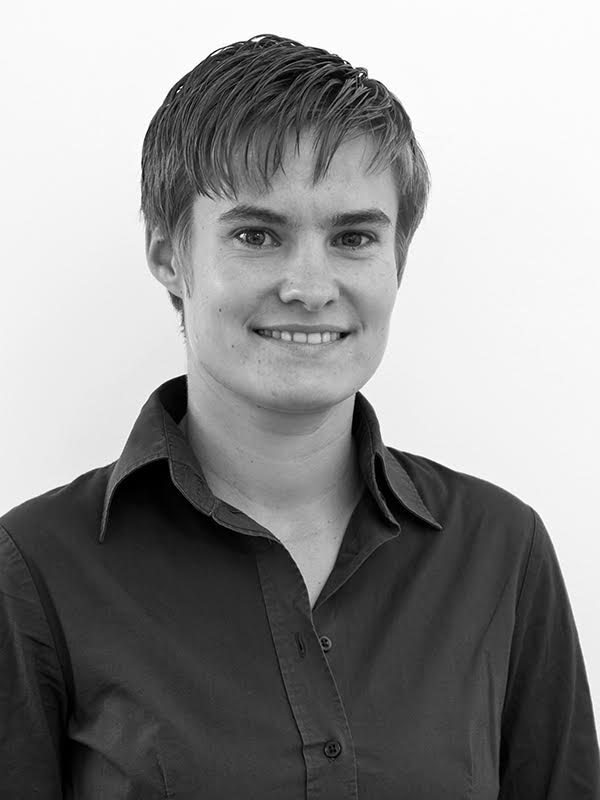
\includegraphics[width=3cm]{behrendt-800.jpg}
  \caption{\textbf{Frauke Behrendt} is Principal Lecturer in Media Studies at the University of Brighton. Her research interests, publications and talks consider digital cultures, sound studies, mobility, interaction design, sustainable transport and smart cities. Behrendt's funded research projects include \lq Smart e-bikes,\rq \lq NetPark\rq and \lq Sonic Interaction Design.\rq Previously, she worked at the University of Sussex, Rhode Island School of Design and Anglia Ruskin University.}
\end{figure}

\begin{figure}[H]
  \sidecaption[t]
  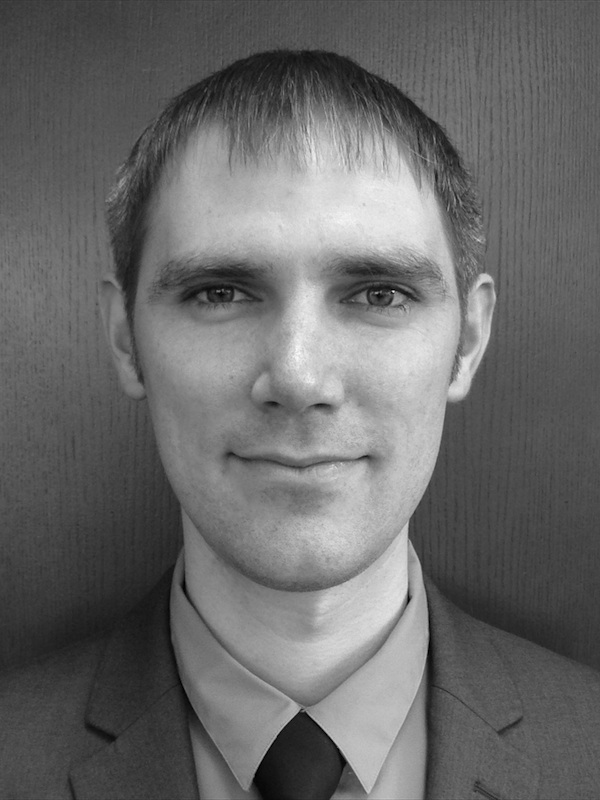
\includegraphics[width=3cm]{berdahl-800.jpg}
  \caption{\textbf{Edgar Berdahl} is Assistant Professor in Experimental Music and Digital Media at Louisiana State University. In collaboration with the Cultural Computing Group at the Center for Computation and Technology, he studies how new technology is influencing new music and vice versa. His research interests include open-source software and hardware, haptics, physical modeling sound synthesis, musical acoustics, algorithmic composition, digital signal processing, sound diffusion systems, embedded musical instruments, feedback control of acoustic musical instruments, and sensing.}
  
  \begin{figure}[H]
  \sidecaption[t]
  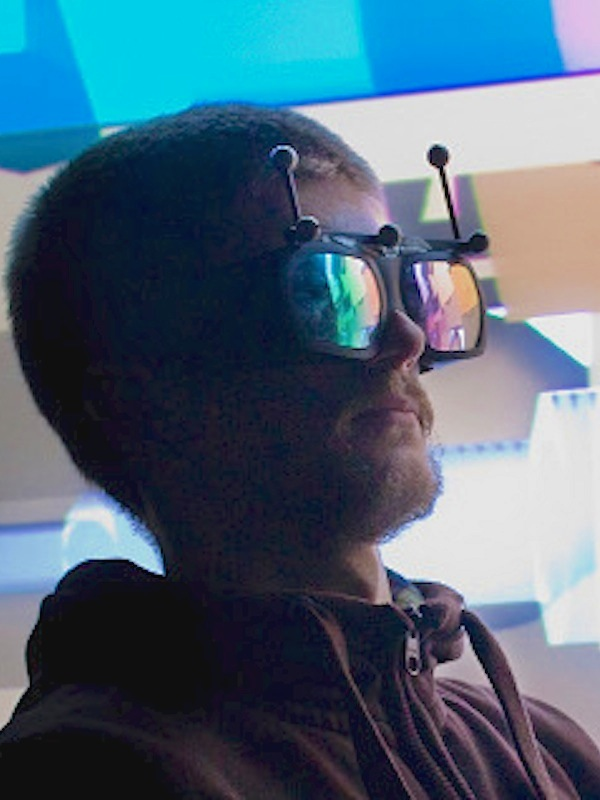
\includegraphics[width=3cm]{berthaut-800.jpg}
  \caption{\textbf{Florent Berthaut} is Assistant Professor at the University of Lille, France and Researcher in the MINT team of CRIStAL. He obtained his PhD in Computer Science from the University of Bordeaux, in the SCRIME/LaBRI and the INRIA Potioc team. He then conducted a two-year project at the University of Bristol with a Marie Curie fellowship. His research focuses on building connections between 3D user interfaces and new interfaces for musical expression. In particular, he has been exploring 3D interaction techniques adapted to musical interaction and mixed-reality display for augmenting digital instruments on stage.}
\end{figure}
\end{figure}

\begin{figure}[H]
  \sidecaption[t]
  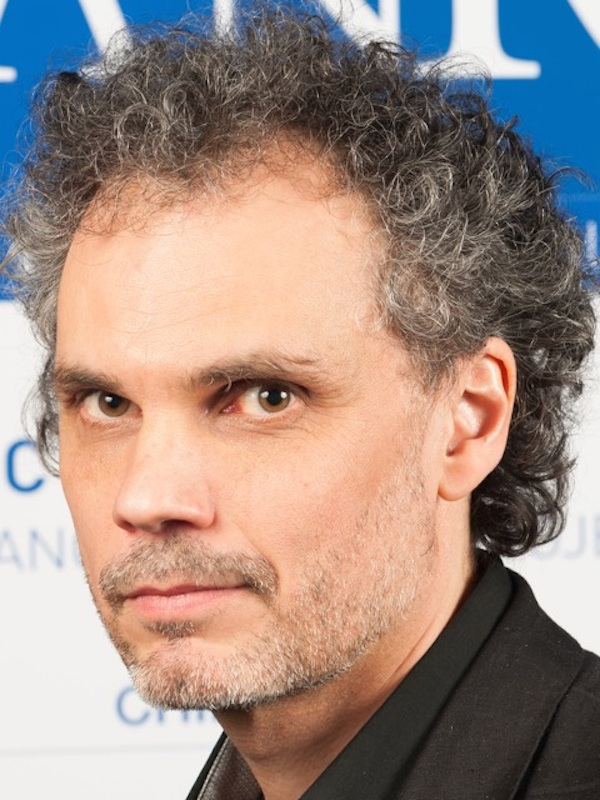
\includegraphics[width=3cm]{bevilacqua-800.jpg}
  \caption{\textbf{Fr\'ed\'eric Bevilacqua} is Head of the Sound Music Movement Interaction team at IRCAM in Paris. His research concerns the modeling of movement--sound interactions, and the design and development of gesture-based interactive systems. He holds a master degree in physics and a PhD in Biomedical Optics from EPFL in Lausanne. From 1999 to 2003 he was a researcher at the University of California, Irvine. In 2003 he joined IRCAM as a researcher on gesture analysis for music and performing arts.}
\end{figure}

\begin{figure}[H]
  \sidecaption[t]
  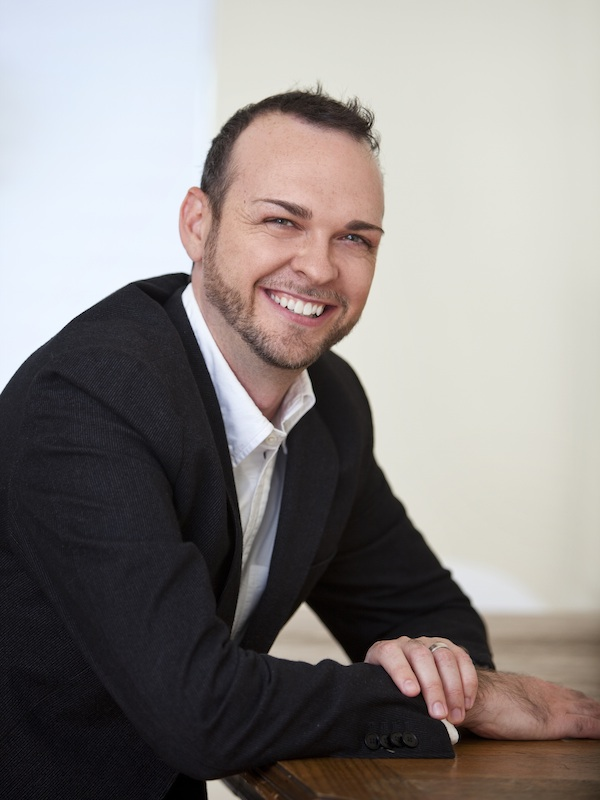
\includegraphics[width=3cm]{birnbaum-800.jpg}
  \caption{\textbf{David Birnbaum} is Design Director at Immersion Corporation, and has been creating haptic experiences for over 10 years. He has worked in the fields of user experience, mobile communication, wearables, gaming, medical devices, and rich interactive media. A leading expert in tactile design, he's driven by a desire to tell stories with the sense of touch and to bring emotion and realism to digital experiences. David holds a BS in Music Industry from USC and a MA in Music Technology from McGill University. He is a named inventor on over 70 patents in the US, Korea, Japan and China.}
\end{figure}

\begin{figure}[H]
  \sidecaption[t]
  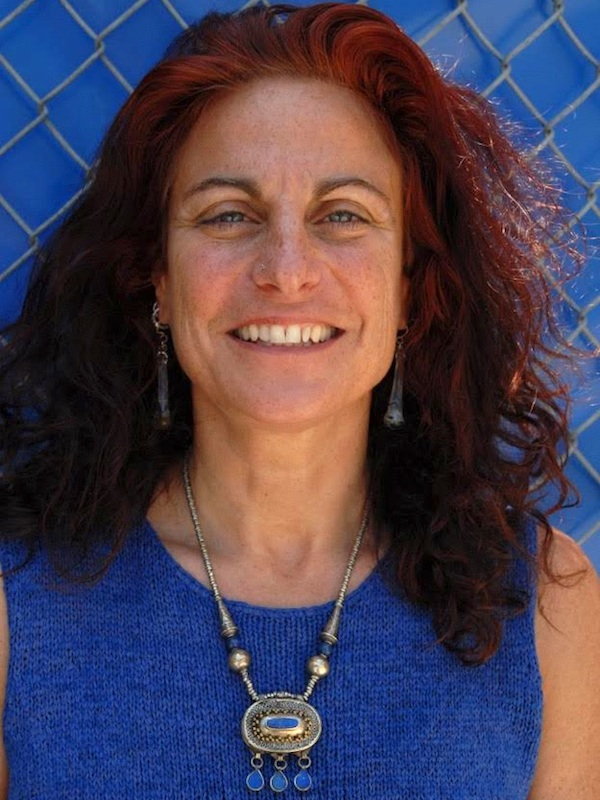
\includegraphics[width=3cm]{blaine-800.jpg}
  \caption{\textbf{Tina Blaine} is a visiting scholar at Carnegie Mellon University's Entertainment Technology Center where she taught for five years, developing collective experiences that integrate game design, sonic discovery and interactive media. Before joining CMU, she worked at Interval Research as a musical interactivist, leading a development team in the creation of the Jam-O-Drum. Blaine is currently the executive director of Rhythmix Cultural Works, a non-profit community theatre/art space in the San Francisco Bay area where people come together to perform, inspire, teach and interact. She is a co-founder of the NIME conference and served as co-artistic director for the Studio for Electro-Instrumental Music in Amsterdam in 2008.}
\end{figure}

\begin{figure}[H]
  \sidecaption[t]
  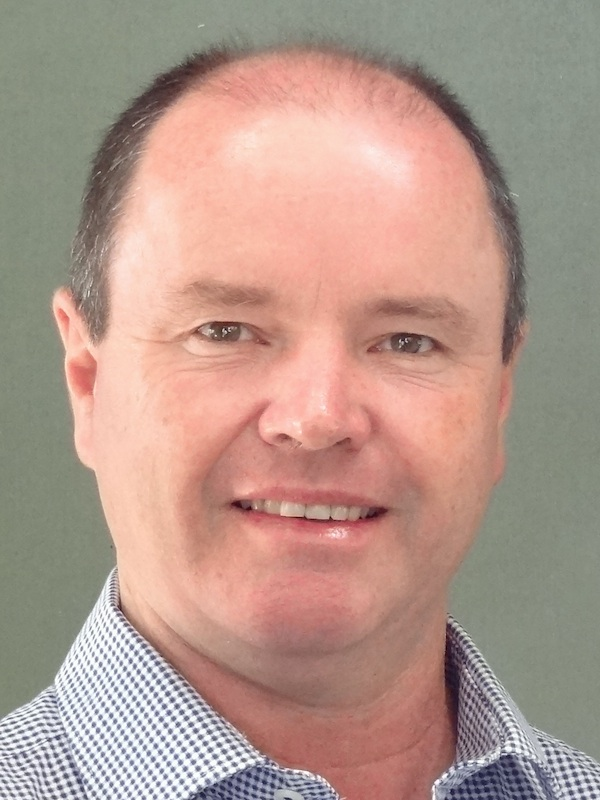
\includegraphics[width=3cm]{brown-800.jpg}
  \caption{\textbf{Andrew R. Brown} is Professor of Digital Arts at Griffith University in Brisbane, Australia. He is an active computer musician and computational artist. His research interests include digital creativity, computational aesthetics, music education and the philosophy of technology. He pursues a creative practice in computer-assisted music performance and audio-visual installations, with focus on generative processes and musical live coding. He is the author of ``Music Technology and Education: Amplifying Musicality,'' co-author of ``Making Music with Computers: Creative Programming in Python,'' and editor of ``Sound Musicianship: Understanding the Crafts of Music.''}
\end{figure}

\begin{figure}[H]
  \sidecaption[t]
  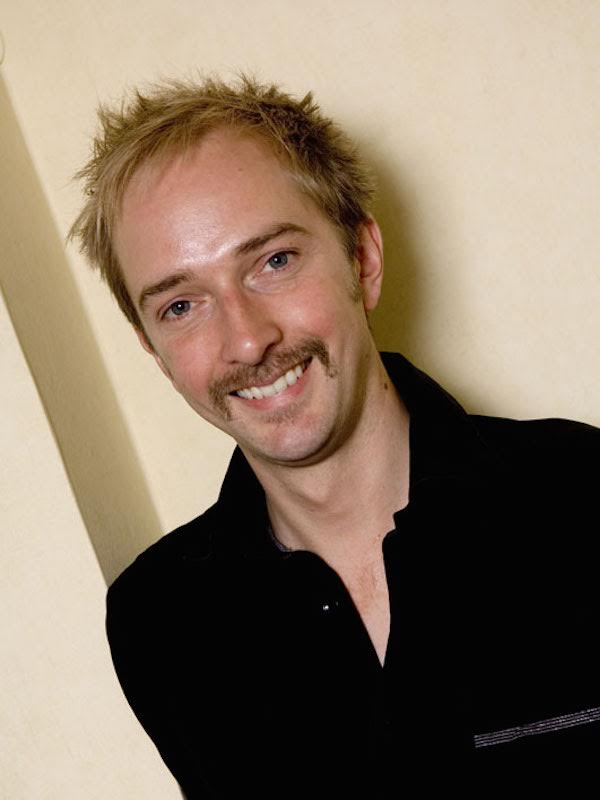
\includegraphics[width=3cm]{bryan-kinns-800.jpg}
  \caption{\textbf{Nick Bryan-Kinns} is Reader in Interaction Design and Deputy Dean at Queen Mary University of London, and Visiting Professor of Interaction Design at Hunan University, China. He leads Interactional Sound and Music at QMUL and has published award winning international journal papers from his multi-million pound funded research. He provided expert opinion for the NSF and European Commission, chaired ACM Creativity and Cognition conference 2009, and BCS-HCI 2006. He is a BCS Fellow, recipient of ACM and BCS Recognition of Service Awards, and founding chair of ACM SIGCHI-CCaA Community. Bryan-Kinns is a Chartered Engineer and received his PhD in 1998.}
\end{figure}

\begin{figure}[H]
  \sidecaption[t]
  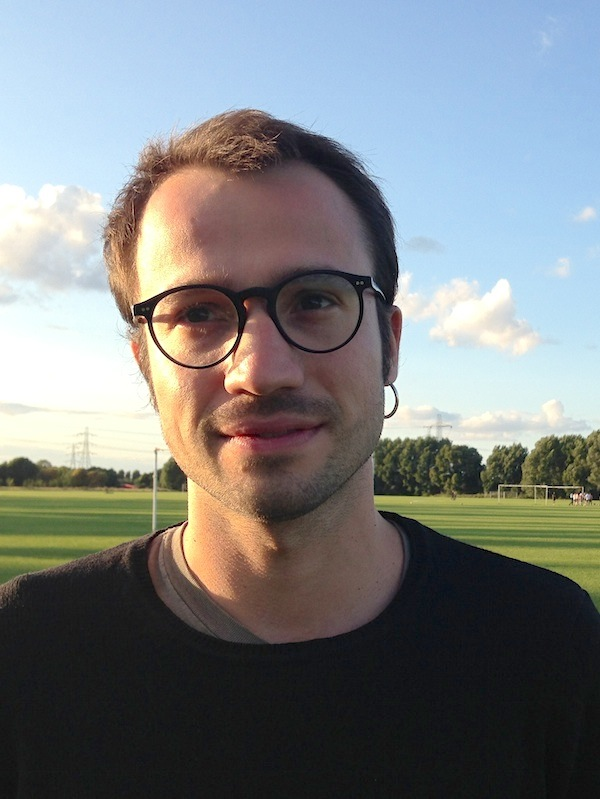
\includegraphics[width=3cm]{caramiaux-800.jpg}
  \caption{\textbf{Baptiste Caramiaux} is a Marie Sklowodska Curie Research Fellow between McGill University and IRCAM. His current research focuses on the understanding of the cognitive processes of motor learning in musical performance and the computational modelling of these processes. Before, he worked on gesture expressivity and the design of musical interactive systems through machine learning. He conducted academic research at Goldsmiths University of London, and applied part of his academic research works on industrial products at Mogees Ltd. Baptiste holds a PhD in computer science from University Pierre et Marie Curie in Paris, and IRCAM Centre Pompidou.}
\end{figure}

\begin{figure}[H]
  \sidecaption[t]
  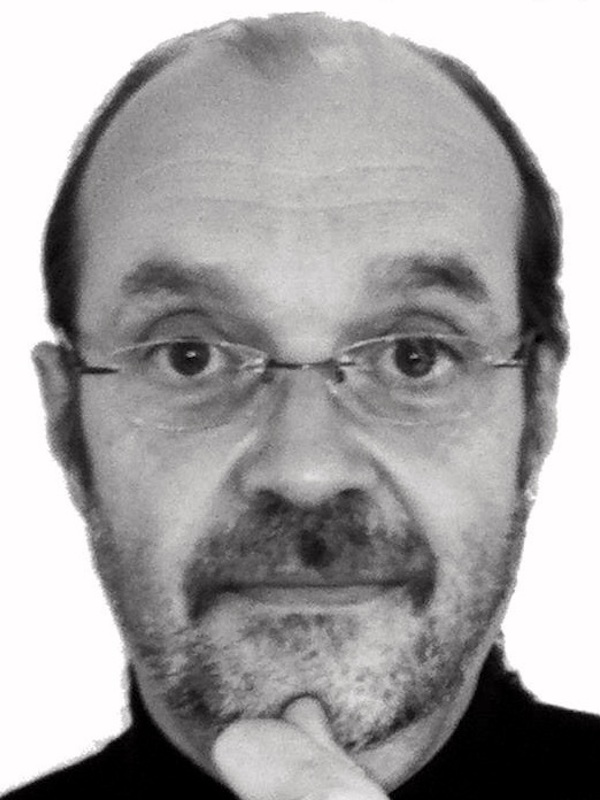
\includegraphics[width=3cm]{cook-800.jpg}
  \caption{\textbf{Perry R. Cook} is Emeritus Professor of Computer Science (also Music) at Princeton University, a founding advisor to music app company Smule, and co-founder/Executive VP of Educational Technology Startup Kadenze, Inc. With Dan Trueman, he co-founded the Princeton Laptop Orchestra, which received a MacArthur Digital Learning Initiative Grant in 2005. With Ge Wang, Cook is co-author of the ChucK Programming Language. His newest book is ``Programming for Digital Musicians and Artists: An Introduction to ChucK,'' with Ajay Kapur, Spencer Salazar, and Ge Wang. The recipient of a 2003 Guggenheim Fellowship, Perry lives in Southern Oregon where he researches, writes, composes, farms sunlight, and eats lots of locally grown food.}
\end{figure}

\begin{figure}[H]
  \sidecaption[t]
  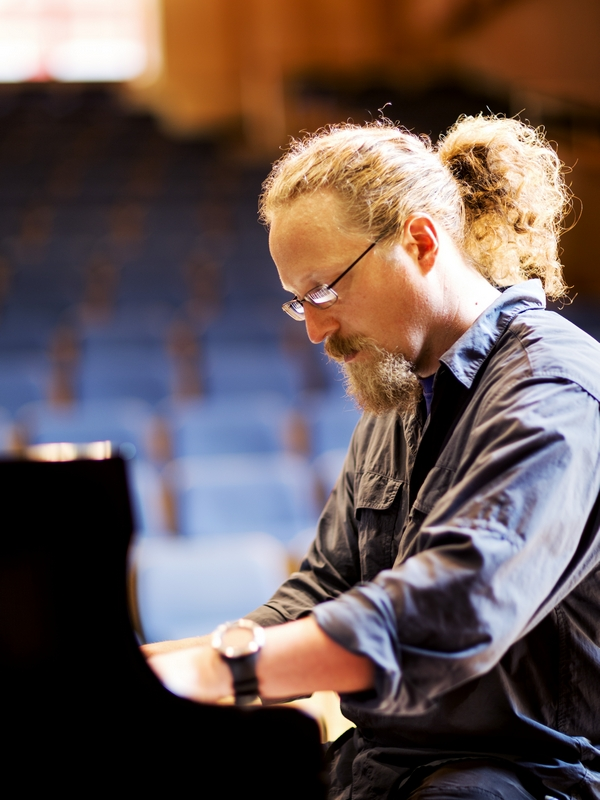
\includegraphics[width=3cm]{dahlstedt-800.jpg}
  \caption{\textbf{Palle Dahlstedt} is a composer, improviser, pianist and researcher. In his research on creative performance technologies, firmly rooted in his artistic practice, he has developed novel mapping algorithms for electronic improvisation, augmented hybrid keyboard instruments, and new kinds of computer-mediated interaction models for improvisers. Dahlstedt has performed solo and with the duo pantoMorf all over the world, and his compositions have been played on six continents. In 2001 he received the Gaudeamus Prize. Currently, Dahlstedt is Obel Professor of Art \& Technology at Aalborg University, Denmark, and Associate Professor of Computer-Aided Creativity and lecturer in composition at University of Gothenburg. Sweden.}
\end{figure}

\begin{figure}[H]
  \sidecaption[t]
  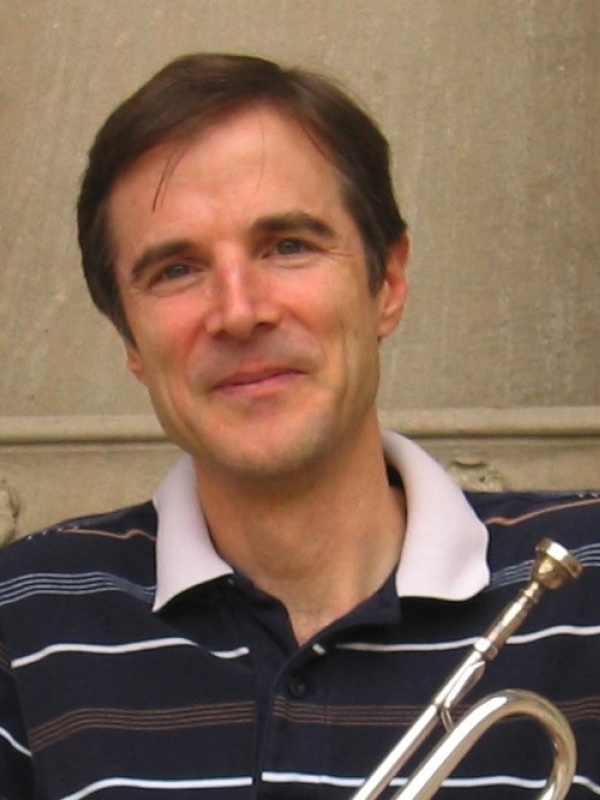
\includegraphics[width=3cm]{dannenberg-800.jpg}
  \caption{\textbf{Roger B. Dannenberg} is Professor of Computer Science in the Schools of Computer Science, Art, and Music at Carnegie Mellon University. Dannenberg has published pioneering work in the areas of interactive systems, computer accompaniment, computer music languages and music education. He is the designer of Nyquist, a language for sound synthesis and music composition, co-creator of Audacity, the audio editor, and as Chief Science Officer to Music Prodigy, the developer of polyphonic pitch recognition software. Dannenberg is also a trumpet player and composer, writing and performing computer and experimental music.}
\end{figure}

\begin{figure}[H]
  \sidecaption[t]
  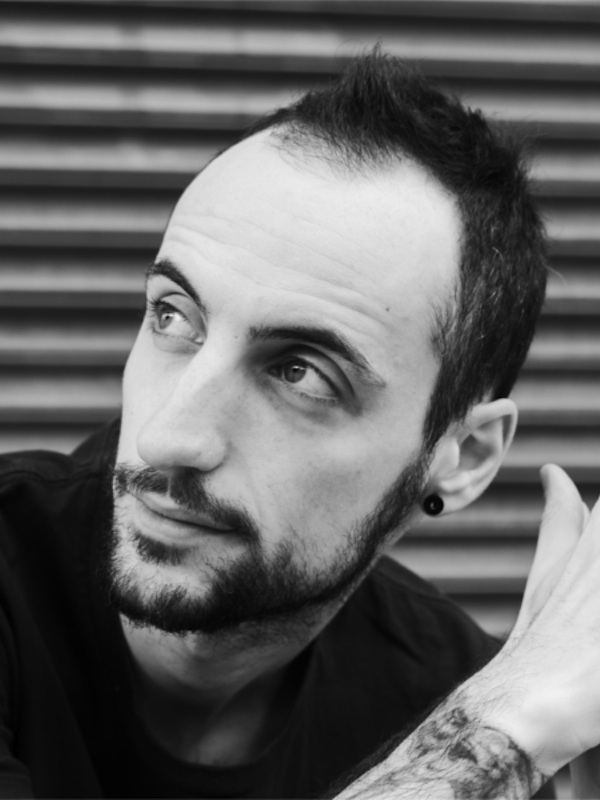
\includegraphics[width=3cm]{donnarumma-800.jpg}
  \caption{\textbf{Marco Donnarumma} is an artist, writer and creator of the biophysical instrument XTH Sense. He creates performances, concerts and installations using and abusing human bodies, sound, infrasound, light, algorithms, body sensors and loudspeakers. His works rely on the material force of sound to produce intensely intimate encounters of bodies and machines, and vivid sensory and physical experiences. His recent practice-based PhD thesis focusses on the politics of corporeality, sound and physiological technologies in musical performance and body art. He has toured over 50 countries and published in leading journals and books. His company, XTH, creates open source biocreative instruments.}
\end{figure}

\begin{figure}[H]
  \sidecaption[t]
  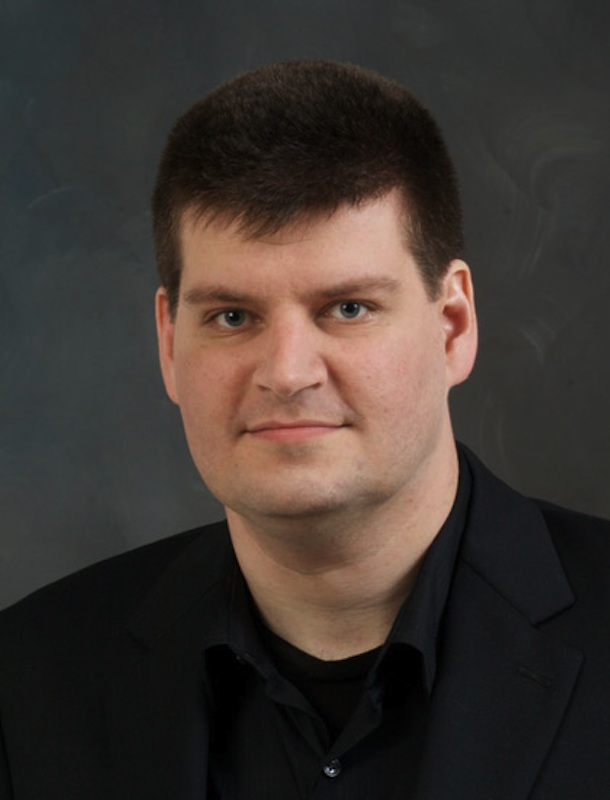
\includegraphics[width=3cm]{essl-800.jpg}
  \caption{\textbf{Georg Essl} is Assistant Professor of Electrical Engineering \& Computer Science as well as Music at the University of Michigan. He received his PhD from Princeton University in 2002 working with Perry Cook on real-time sound synthesis method for solid objects. After a year on the faculty of University of Florida he worked at MIT Media Lab Europe with Sile O'Modhrain on tangible user interfaces. Then, at Deutsche Telekom Laboratories, he started to turn mobile phones into musical instruments. He is founding director of a number of Mobile Phone Orchestras and Ensembles including Stanford, Berlin, and Michigan.}
\end{figure}

\begin{figure}[H]
  \sidecaption[t]
  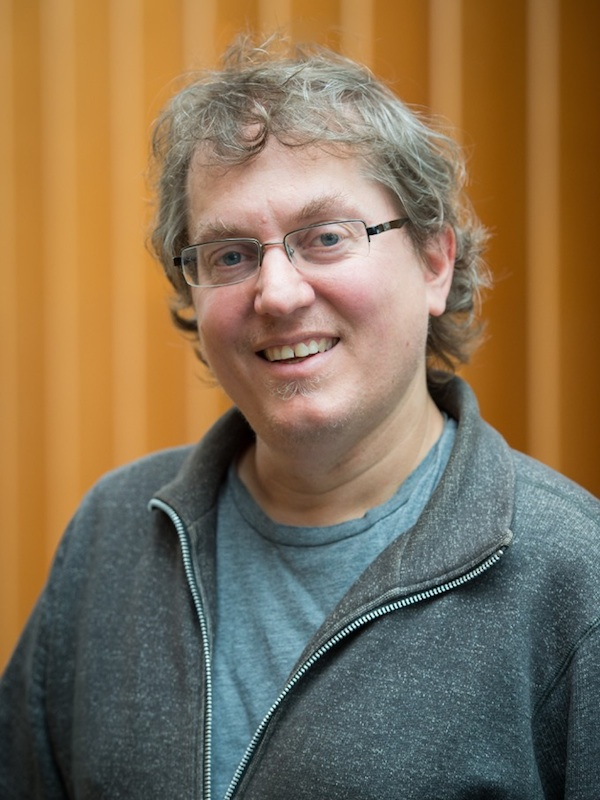
\includegraphics[width=3cm]{fels-800.jpg}
  \caption{\textbf{Sid Fels} is a Distinguished University Scholar at The University of British Columbia (2004--). He was a visiting researcher at ATR Media Integration \& Communications Research Laboratories in Kyoto, Japan (1996--1997). He is internationally known for his work in human-computer interaction, biomechanical modeling, neural networks, new interfaces for musical expression and interactive arts with over 250 scholarly publications. Fels is the academic lead on the biomechanical modeling efforts for the Parametric Human project and leads a collaborative health research project on modeling swallowing. He is one of the co-founders of NIME. }
\end{figure}

\begin{figure}[H]
  \sidecaption[t]
  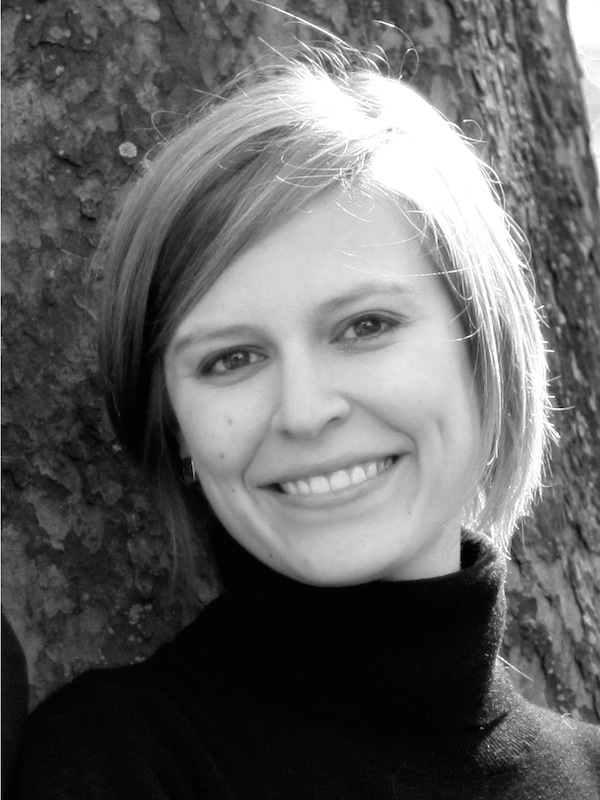
\includegraphics[width=3cm]{fiebrink-800.jpg}
  \caption{\textbf{Rebecca Fiebrink} is Lecturer at Goldsmiths, University of London. Her research focuses on designing new ways for humans to interact with computers in creative practice, and she is the developer of the Wekinator software for interactive machine learning. She has worked with companies including Microsoft Research, Sun Microsystems Research Labs, Imagine Research, and Smule, where she helped to build the \#1 iTunes app ``I am T-Pain.'' She holds a PhD in Computer Science from Princeton University. Prior to moving to Goldsmiths, she was an assistant professor at Princeton University, where she co-directed the Princeton Laptop Orchestra.}
\end{figure}


\begin{figure}[H]
  \sidecaption[t]
  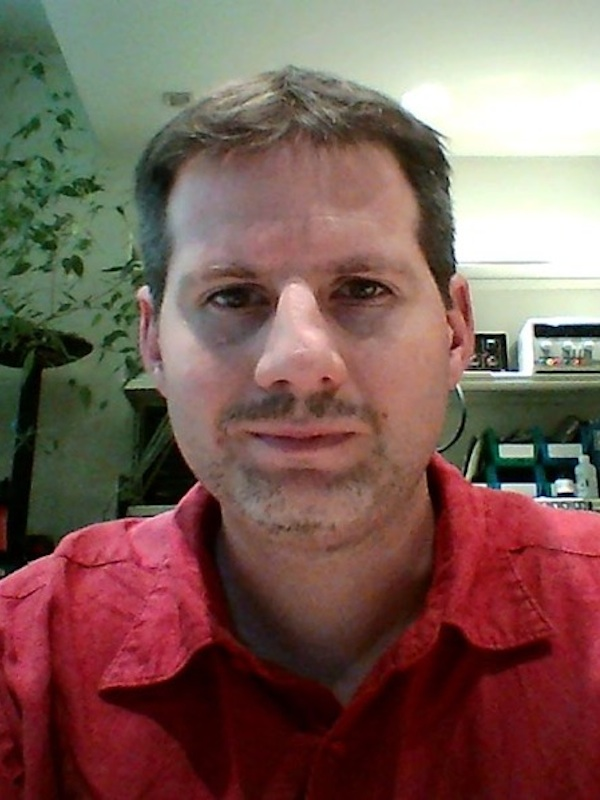
\includegraphics[width=3cm]{flety-800.jpg}
  \caption{\textbf{Emmanuel Fl\'ety} is an electronic engineer at IRCAM in Paris. He leads the hardware design for both research and art applications, focusing on wireless sensor technologies and gestural interaction. He holds a degree in electronic engineering from ENSEA and joined IRCAM in 1999 to develop stage interaction for performing arts.}
\end{figure}

\begin{figure}[H]
  \sidecaption[t]
  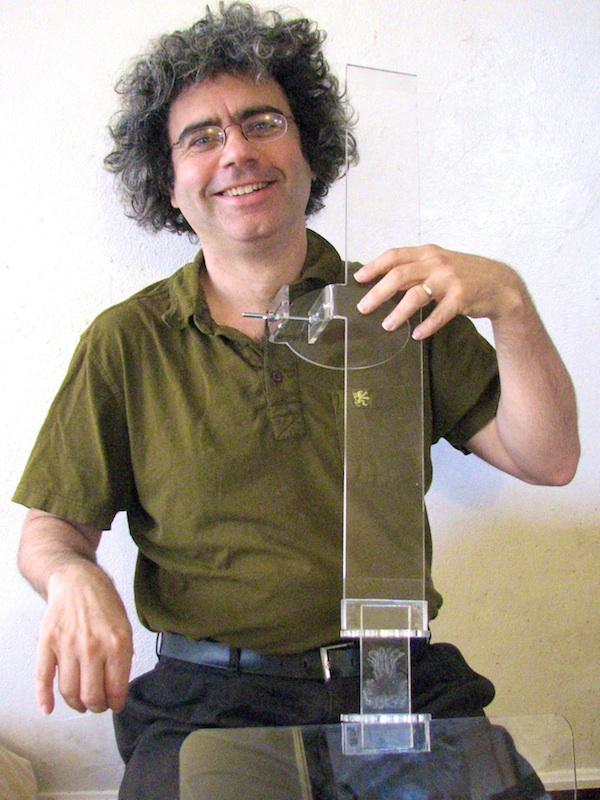
\includegraphics[width=3cm]{freed-800.jpg}
  \caption{\textbf{Adrian Freed} is Research Director of UC Berkeley's Center for New Music and Audio Technologies (CNMAT). He has pioneered many new applications of mathematics, electronics and computer science to audio, music and media production tools including the first graphical user interfaces for digital sound editing, mixing and processing. He invented the audio plug-in, and co-invented Open Sound Control. (OSC). His current work involves movement and intermedia, gesture signal processing, and terra-scale integration of data from wearable and built environment sensor/actuator systems using printed electronics, electro-textiles and other emerging materials.}
\end{figure}

\begin{figure}[H]
  \sidecaption[t]
  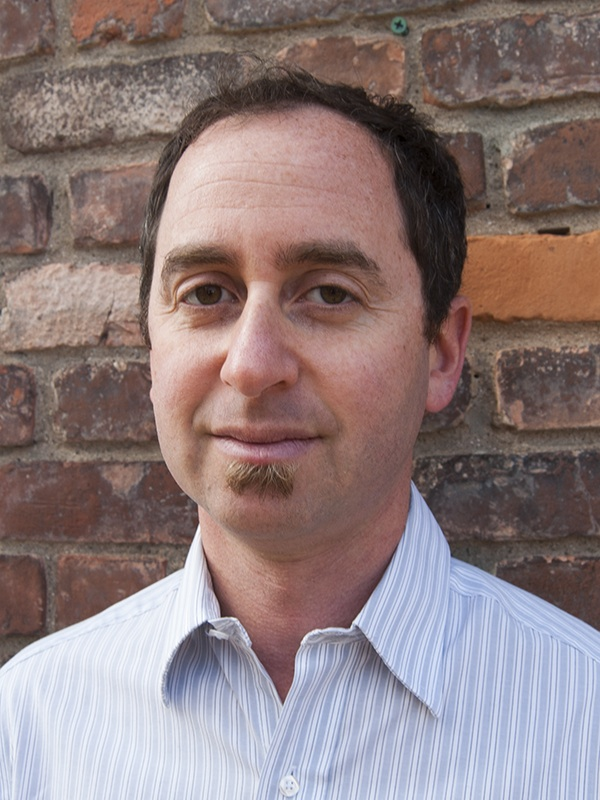
\includegraphics[width=3cm]{gurevich-800.jpg}
  \caption{\textbf{Michael Gurevich} is Assistant Professor of Performing Arts Technology at the University of Michigan's School of Music, Theatre \& Dance. His research explores new aesthetic and interactional possibilities that can emerge in performance with real-time computer systems. Other research areas include network-based music performance, computational acoustic modeling of bio-acoustic systems, and historical aspects of computer music. His creative practice explores many of the same themes, through experimental compositions involving interactive media, sound installations, and the design of new musical interfaces. At Michigan, he directs an ensemble dedicated to the performance of electronic chamber music.}
\end{figure}

\begin{figure}[H]
  \sidecaption[t]
  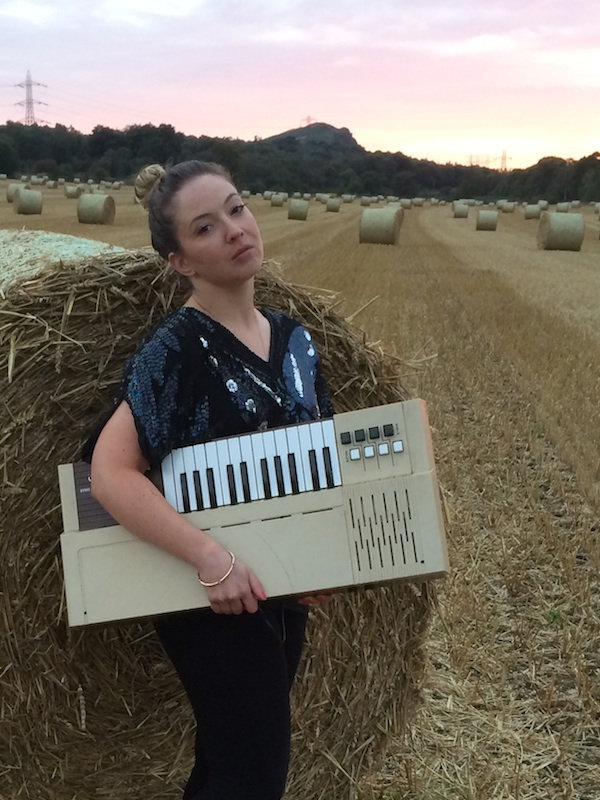
\includegraphics[width=3cm]{hayes-800.jpg}
  \caption{\textbf{Lauren Sarah Hayes} is a Scottish musician and sound artist who creates physical live electronic music. She is a regular improviser on both augmented piano and analogue/digital hybrid electronics. Her research examines the links between sound and touch and she has developed and performed with bespoke haptic and vibro-tactile devices over a prolonged period of creative practice. Her work has been presented globally at festivals and within publications such as Organised Sound and Contemporary Music Review. She is currently Assistant Professor of Sound Studies at Arizona State University and an associate of the New Radiophonic Workshop.}
\end{figure}

\begin{figure}[H]
  \sidecaption[t]
  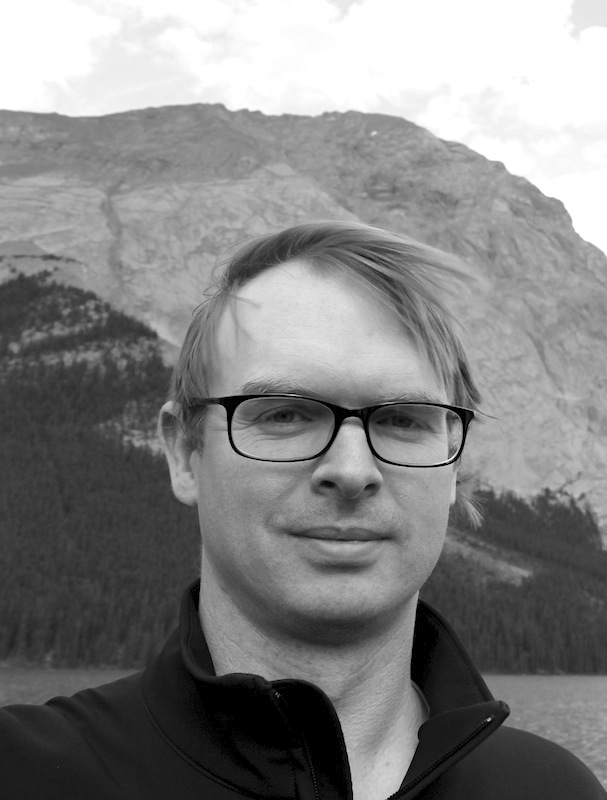
\includegraphics[width=3cm]{hindle-800.jpg}
  \caption{\textbf{Abram Hindle} is an assistant professor of Computing Science at the University of Alberta. His research focuses on problems relating to mining software repositories, improving software engineering-oriented information retrieval with contextual information, the impact of software maintenance on software energy consumption, and how software engineering informs computer music. Abram received a PhD in computer science from the University of Waterloo.}
\end{figure}

\begin{figure}[H]
  \sidecaption[t]
  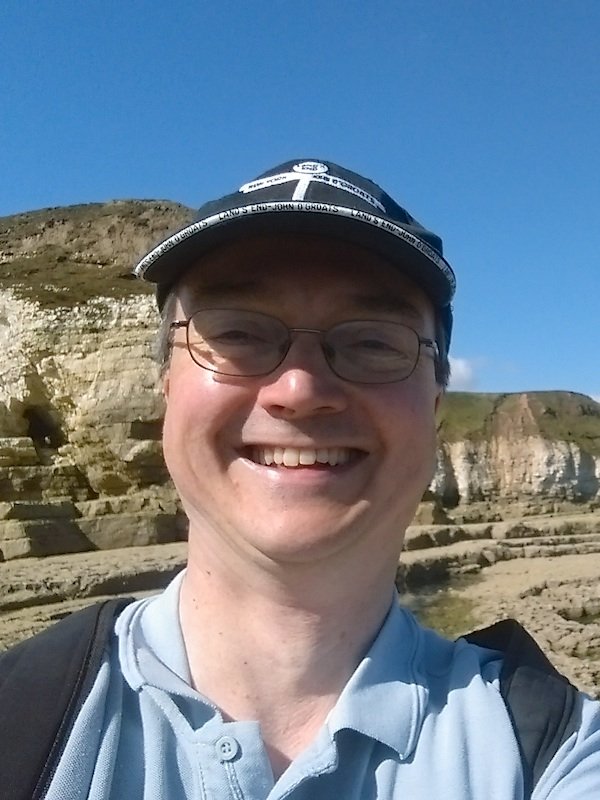
\includegraphics[width=3cm]{hunt-800.jpg}
  \caption{\textbf{Andy Hunt} is Professor and Deputy Head (Teaching \& Scholarship) in the Department of Electronics at the University of York UK. He worked on York's first Music Technology courses in 1988 and has developed the teaching there since that date. His special interests include the use of sound to portray data (sonification), and the human-computer interface for interactive performance instruments. Over the last decade Andy has worked with Thomas Hermann and Roberto Bresin to push forward the field of \emph{interactive sonification}, which is a blend of the two interests (HCI and auditory display). He is co-editor of ``The Sonification Handbook.''}
\end{figure}

\begin{figure}[H]
  \sidecaption[t]
  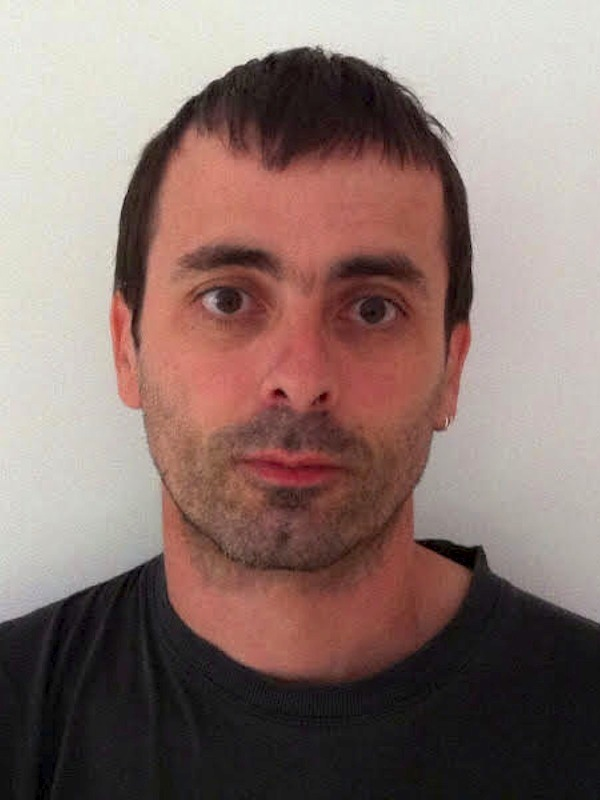
\includegraphics[width=3cm]{hurtado-800.jpg}
  \caption{\textbf{Enrike Hurtado} is a researcher at the University of Bilbao, and is currently exploring the digitalisation of the txalaparta, an ancient basque percussion tradition. Enrike's background is in fine arts and he has been strongly involved in experimental music working with improvisation, electronic music and experimental rock. He is co-founder of ixi audio where he has developed experimental software and taught workshops in the creative use of programming. His interest ranges from process based music to improvisational rule based systems and live coding.}
\end{figure}

\begin{figure}[H]
  \sidecaption[t]
  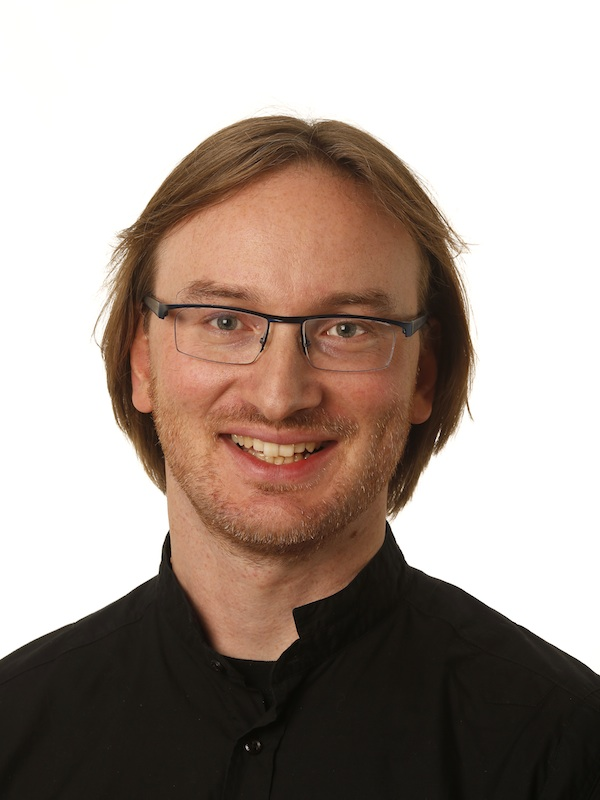
\includegraphics[width=3cm]{jensenius-800.jpg}
  \caption{\textbf{Alexander Refsum Jensenius} is a music researcher and research musician working at the Department of Musicology, University of Oslo. He studied at the University of Oslo and Chalmers University of Technology and have been a visiting researcher at CNMAT, UC Berkeley and CIRMMT, McGill University. His research focuses on music-related body motion, from both analytical and creative perspectives. Alexander organized the NIME 2011 conference and is currently chair of the NIME steering committee.}
\end{figure}

\begin{figure}[H]
  \sidecaption[t]
  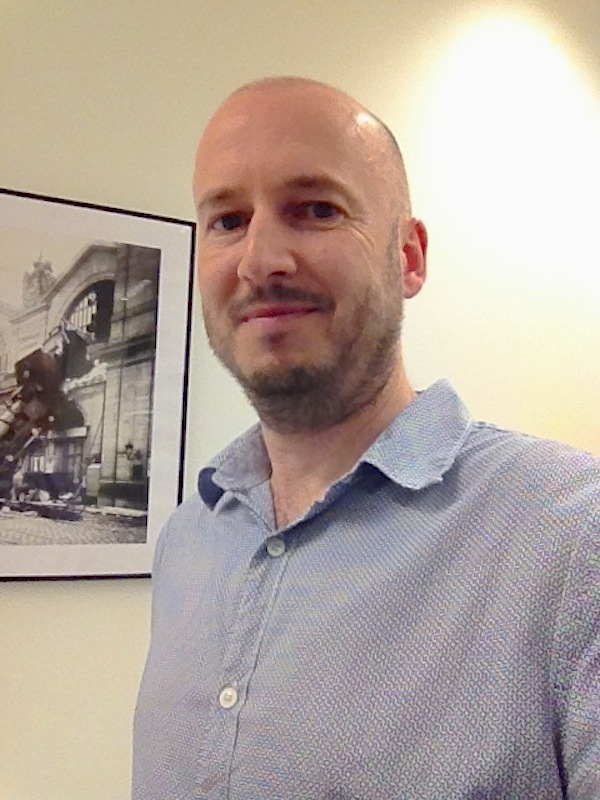
\includegraphics[width=3cm]{johnston-800.jpg}
  \caption{\textbf{Andrew Johnston} is a researcher, interaction/software designer and musician based in Sydney, Australia. His work focuses on the design of systems that support experimental, exploratory approaches to live performance, and the experiences of the artists who use them. Andrew is co-director of the Creativity and Cognition Studios, an interdisciplinary research group working at the intersection of creativity and technology. He currently holds the position of Senior Lecturer in the School of Software, Faculty of Engineering and IT at the University of Technology Sydney. }
\end{figure}

\begin{figure}[H]
  \sidecaption[t]
  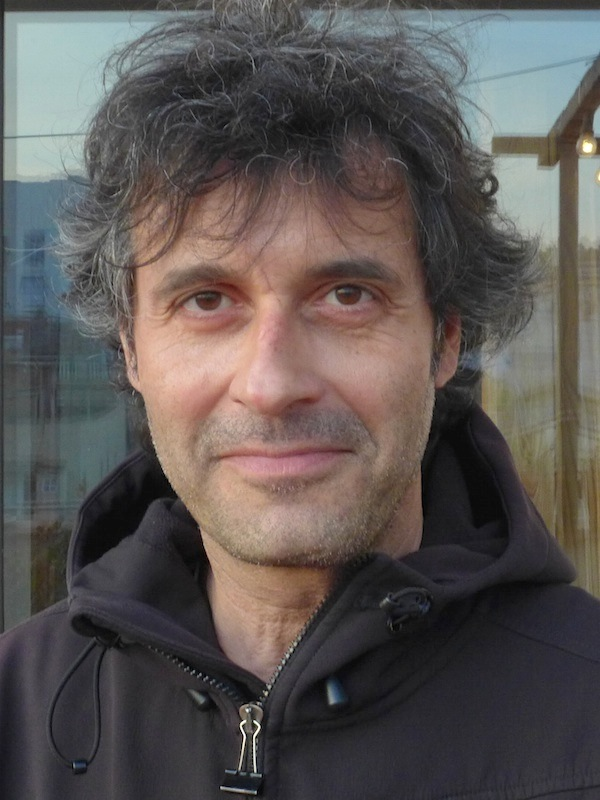
\includegraphics[width=3cm]{jorda-800.jpg}
  \caption{\textbf{Sergi Jord\`{a}} holds a BS in Fundamental Physics and a PhD in Computer Science and Digital Communication. He is a researcher at the Music Technology Group, Universitat Pompeu Fabra, where he directs the Music and Multimodal Interaction Lab. In the early 1980s, after discovering programming, he devoted himself to computer music improvisation. Throughout the 1990s he developed interactive installations and multimedia performances, and re-entered academia by the end of the millennium. His main research interests are in the confluence of HCI, tangible, musical and physiological interaction. He has received several international awards, including the Prix Ars Electronica Golden Nica (2008).}
\end{figure}

\begin{figure}[H]
  \sidecaption[t]
  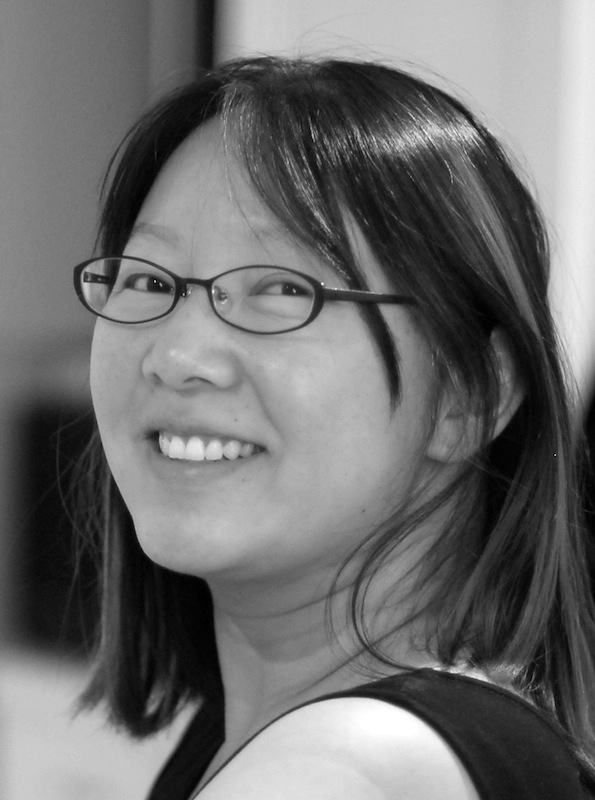
\includegraphics[width=3cm]{ju-800.jpg}
  \caption{\textbf{Wendy Ju} is Executive Director for Interaction Design Research at Stanford's Center for Design Research, and an Associate Professor in the Graduate Design Program at the California College of the Arts in San Francisco. Her research is primarily focused on the design of interactive devices, particularly human-robot interaction and autonomous car interfaces. She received her Master's degree from the MIT Media Lab in 2001, and her doctorate from Stanford University in 2008. She is the author of the book ``The Design of Implicit Interactions,'' which is available from Morgan and Claypool.}
\end{figure}

\begin{figure}[H]
  \sidecaption[t]
  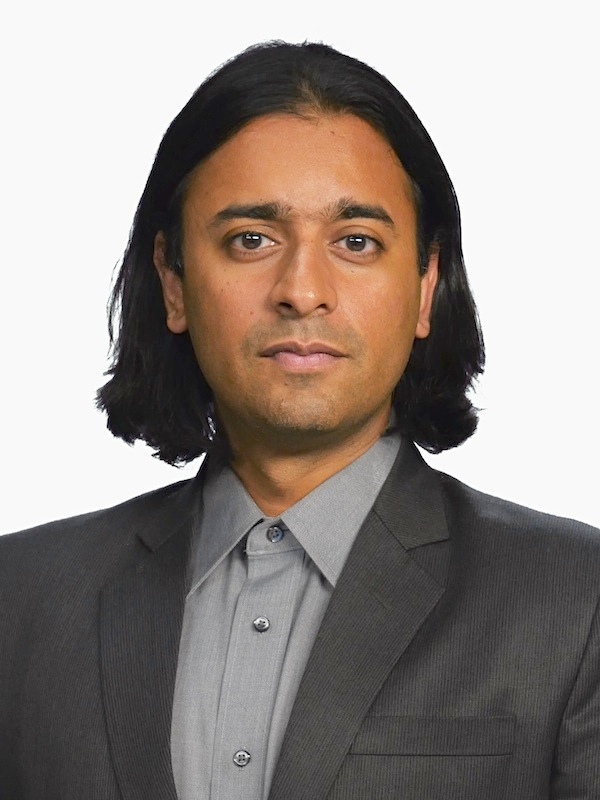
\includegraphics[width=3cm]{kapur-800.jpg}
  \caption{\textbf{Ajay Kapur} is Director of the Music Technology program (MTIID) at the California Institute of the Arts, as well as the Associate Dean for Research and Development in Digital Arts. He runs a PhD Research Group in Wellington New Zealand called Sonic Engineering Lab for Creative Technology. He is also Founder and CEO of Kadenze, the Creative Arts MOOC. Kapur has published over 100 technical papers and presented lectures across the world on music technology, human computer interface for artists, robotics for making sound, and modern digital orchestras.}
\end{figure}

\begin{figure}[H]
  \sidecaption[t]
  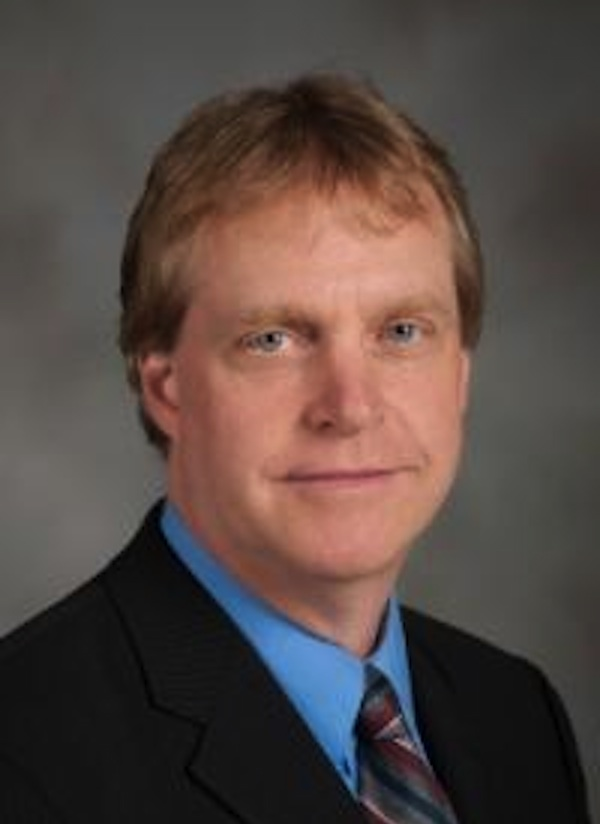
\includegraphics[width=3cm]{knapp-800.jpg}
  \caption{\textbf{R. Benjamin Knapp} is the Director of the Institute for Creativity, Arts, and Technology (ICAT) and Professor of Computer Science at Virginia Tech. ICAT seeks to promote research and education at the boundaries between art, design, engineering, and science. For more than 20 years, Dr. Knapp has been working to create meaningful links between human-computer interaction, universal design, and various forms of creativity. His research on human-computer interaction has focused on the development and design of user-interfaces and software that allow both composers and performers to augment the physical control of a musical instrument with direct sensory interaction.}
\end{figure}

\begin{figure}[H]
  \sidecaption[t]
  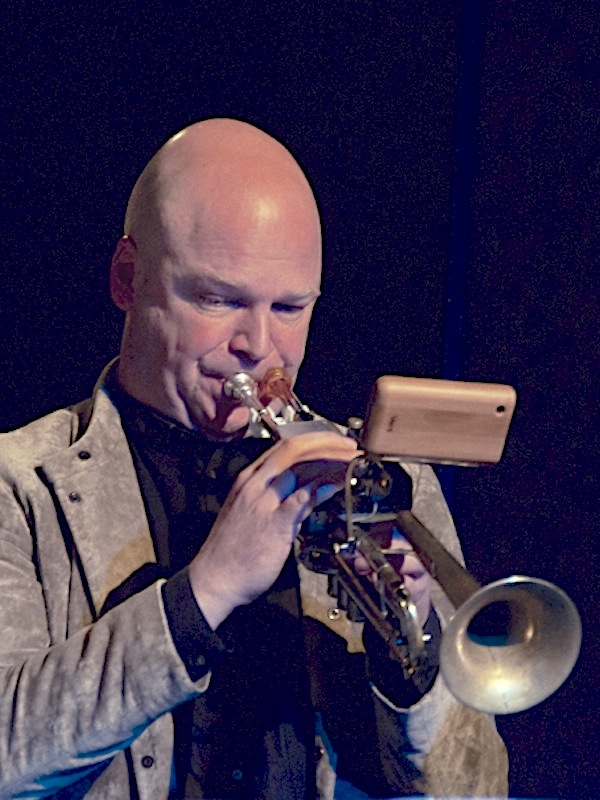
\includegraphics[width=3cm]{leeuw-800.jpg}
  \caption{\textbf{Hans Leeuw} is a trumpet player, composer and band leader from the Netherlands. He led and got commissioned (by the Dutch art council) for the 15-piece big band Tetzepi between 1997 and 2014. This band was successful within the Dutch avant garde Jazz scene and toured through the Netherlands as well as Europe. In 2008 Hans started to develop the Electrumpet with which he won the international Guthman competition for new musical instruments in Atlanta in 2013. Hans is a senior Lecturer at the University of the Arts Utrecht since 1993 and started a PhD in Huddersfield with Professor Pierre Alexandre Tremblay in 2014.}
\end{figure}


\begin{figure}[H]
  \sidecaption[t]
  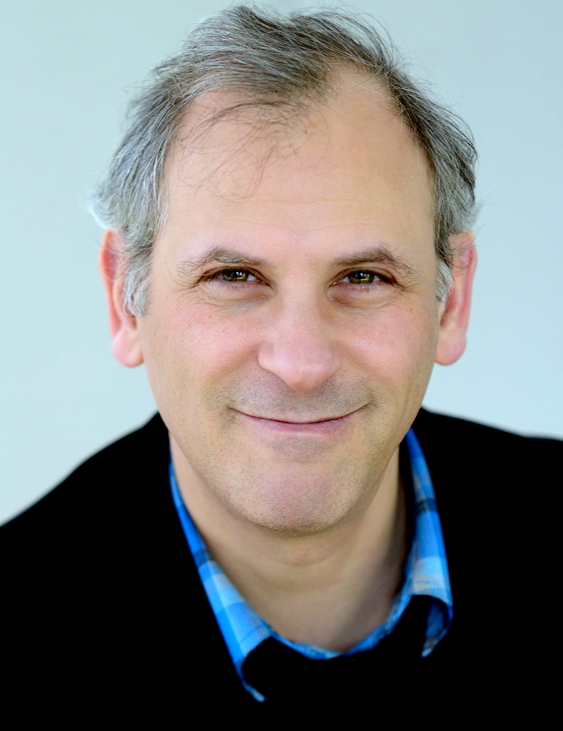
\includegraphics[width=3cm]{lyon-800.jpg}
  \caption{\textbf{Eric Lyon} is a composer and computer music researcher who focuses on articulated noise, spatial orchestration and computer chamber music. His software includes FFTease and LyonPotpourri. He is the author of ``Designing Audio Objects for Max/MSP and Pd,'' which explicates the process of designing and implementing audio DSP externals. His music has been selected for the Giga-Hertz prize, MUSLAB, and the ISCM World Music Days. Lyon has taught computer music at Keio University, IAMAS, Dartmouth, Manchester University, and Queen’s University Belfast. Currently, he teaches at Virginia Tech, and is a faculty fellow at the Institute for Creativity, Arts, and Technology.}
\end{figure}

\begin{figure}[H]
  \sidecaption[t]
  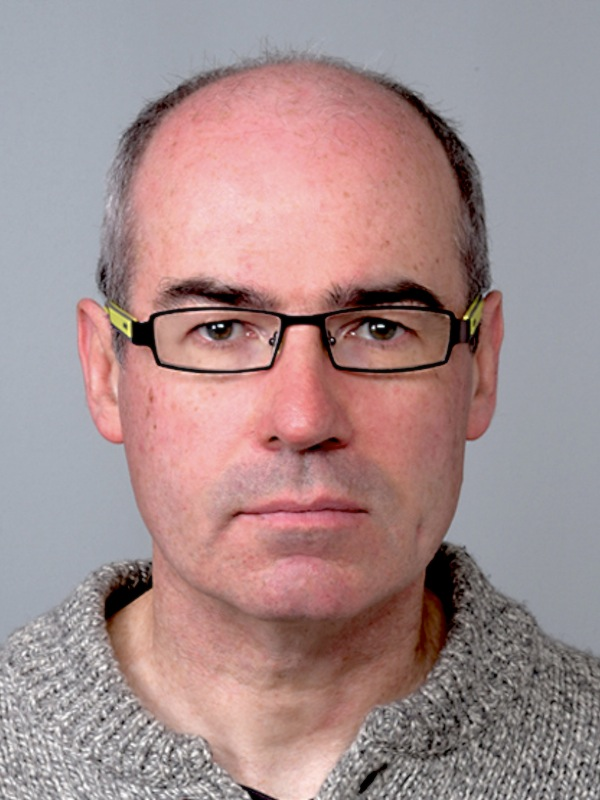
\includegraphics[width=3cm]{lyons-800.jpg}
  \caption{\textbf{Michael Lyons} is Professor of Image Arts and Sciences at Ritsumeikan University. He studied physics at McGill University (BSc) and the University of British Columbia (MSc, PhD). He has worked in computational neuroscience, pattern recognition, human-computer interaction, and media arts, as a Research Fellow at the California Institute of Technology, Research Assistant Professor at the University of Southern California, and Senior Research Scientist at the ATR Research Labs. Michael proposed and co-organized the CHI 2001 workshop on New Interfaces for Musical Expression, and has served as a founding member of the NIME steering committee and advisory board.}
\end{figure}

\begin{figure}[H]
  \sidecaption[t]
  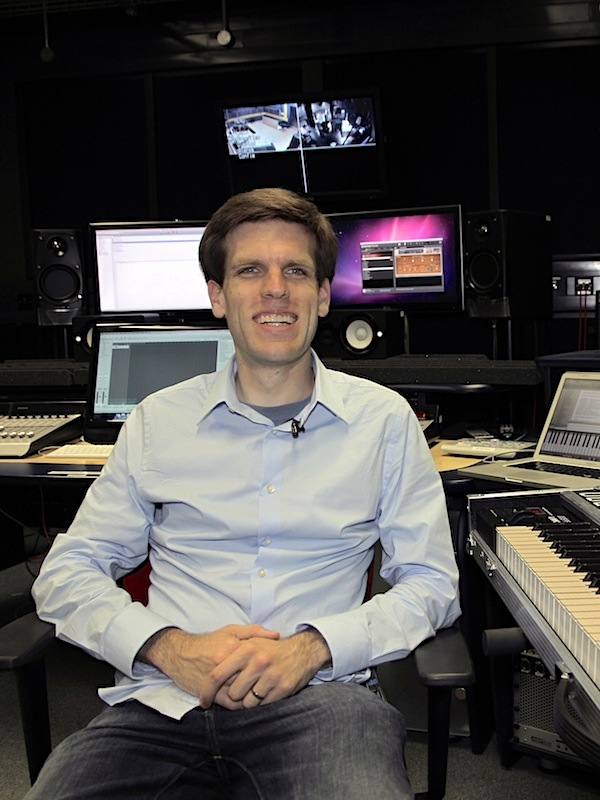
\includegraphics[width=3cm]{mcpherson-800.jpg}
  \caption{\textbf{Andrew McPherson} is Senior Lecturer (Associate Professor) in the Centre for Digital Music at Queen Mary University of London. A composer and electrical engineer by training, he studied at MIT (M.Eng. 2005) and the University of Pennsylvania (PhD 2009) and spent a two-year postdoctoral fellowship at Drexel University. His research focuses on augmented instruments, embedded hardware systems, the study of performer--instrument interaction and user appropriation of technology. He is the creator of the magnetic resonator piano, an augmented acoustic piano which has been used by more than 20 composers worldwide, and the TouchKeys multi-touch keyboard which successfully launched on Kickstarter in 2013.}
\end{figure}

\begin{figure}[H]
  \sidecaption[t]
  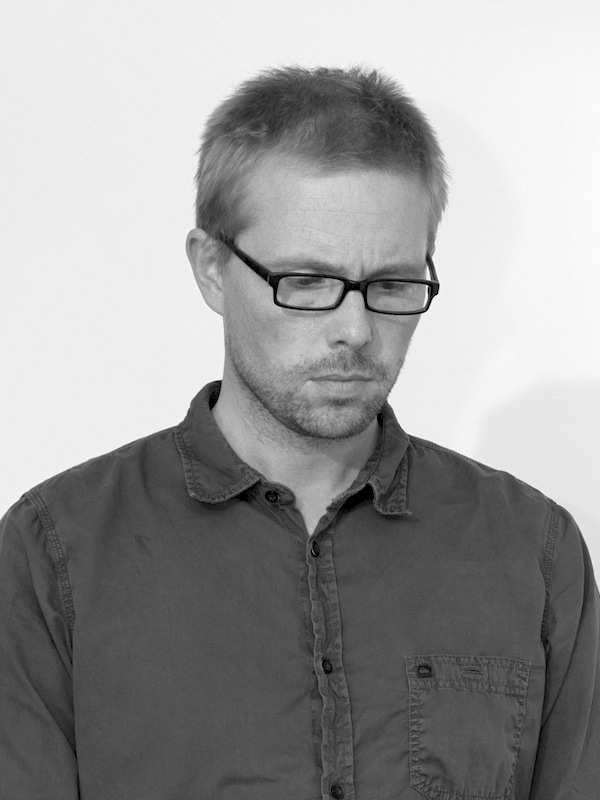
\includegraphics[width=3cm]{magnusson-800.jpg}
  \caption{\textbf{Thor Magnusson} is a musician and software developer who lectures in music at the University of Sussex. His research focusses on the impact digital technologies have on musical creativity and practice, explored through software development, composition, and performance. He is the co-founder of ixi audio, and has developed audio software, systems of generative music composition, written computer music tutorials, and created two musical live coding environments. As part of ixi, he has taught workshops in creative music coding and sound installations and given presentations, performances, and visiting lectures at diverse art institutions, conservatories, and universities internationally.}
\end{figure}

\begin{figure}[H]
  \sidecaption[t]
  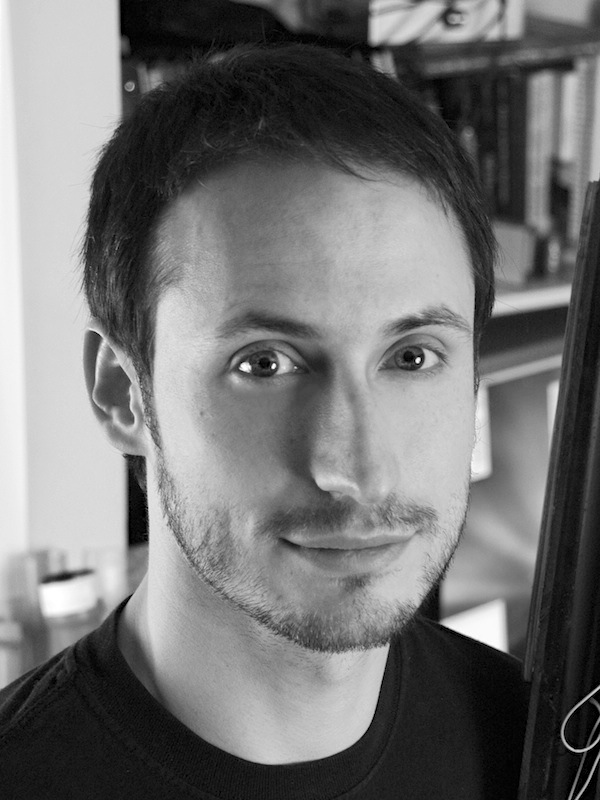
\includegraphics[width=3cm]{malloch-800.jpg}
  \caption{\textbf{Joseph Malloch} is a researcher and instrument designer based in Paris at Inria Saclay/Universit\'e Paris-Sud/CNRS. His research focuses on the design and use of new interfaces for live music performance, tools for supporting collaborative design of interactive systems, and methods for enriching human-computer interactions. He is also the designer/developer of several digital musical instruments, which have appeared in public performances around the world, including performances at new music festivals, international conferences, performances by dancers, and by blind performers in a larger ensemble.}
\end{figure}

\begin{figure}[H]
  \sidecaption[t]
  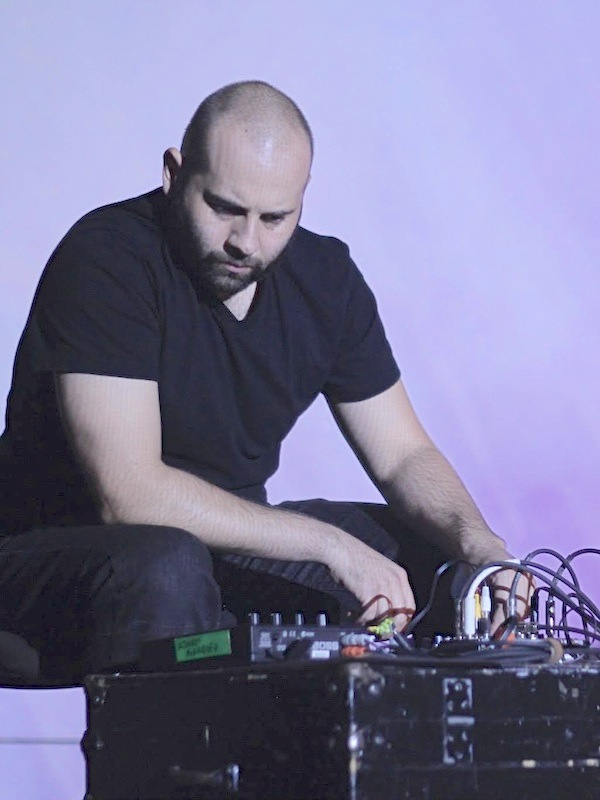
\includegraphics[width=3cm]{marquez-borbon-800.jpg}
  \caption{\textbf{Adnan Marquez-Borbon} is a Mexican improviser, instrument designer, sound artist, and researcher. Currently involved in the interdisciplinary project \lq Into the Key of Law: Transposing Musical Improvisation. The Case of Child Protection in Northern Ireland.\rq The music released under his name synthesises electronic music, jazz, free improvisation, and ethnic musics. His alter ego, duplex helix, produces beat-based music influenced by Hip Hop and various electronic music genres. He is a cofounder of the Mexican improvisation collective Generaci\'on Espont\'{a}nea and the multimedia collective NOR73 (now OpenL4B.Norte\_Hackerspace).}
\end{figure}

\begin{figure}[H]
  \sidecaption[t]
  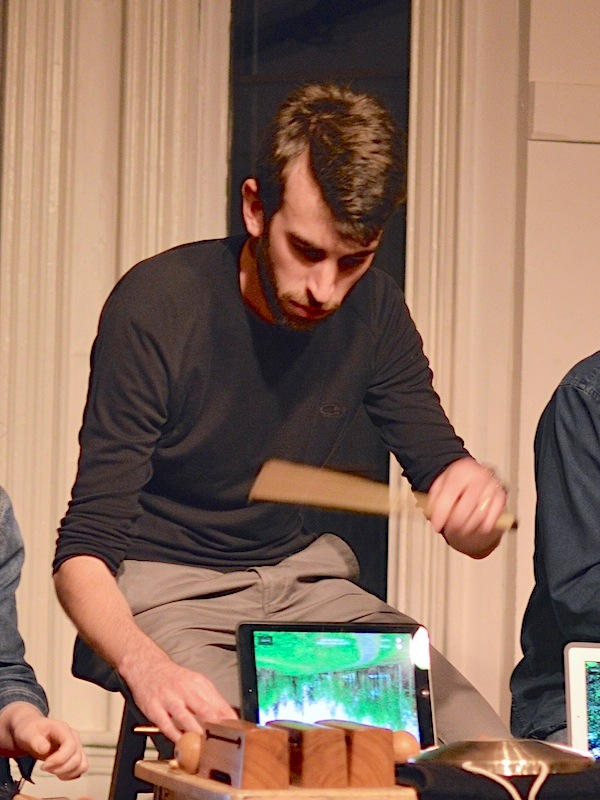
\includegraphics[width=3cm]{martin-800.jpg}
  \caption{\textbf{Charles Martin} is a specialist in percussion, computer music, and human-computer interaction from Canberra, Australia. He links percussion with electroacoustic music and other media through new technologies. His works, described as ``a thing of rare beauty'' in The West Australian, have been performed throughout Australia, Europe and the USA and presented at international conferences on computer music and percussion. Charles has released touch-screen apps for making music and is active in creating performances, workshops and research that explore the musical potential of new computing devices.}
\end{figure}

\begin{figure}[H]
  \sidecaption[t]
  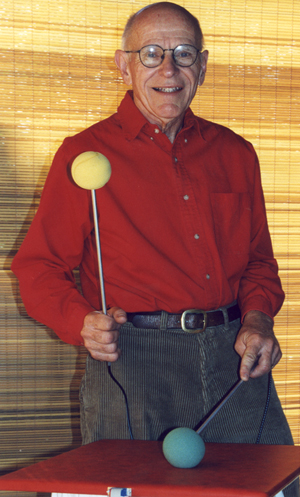
\includegraphics[width=3cm]{mathews.jpg}
  \caption{\textbf{Max Mathews} (1926--2011) was a music technology pioneer and is often called the ``father of computer music'' after writing the first version of *Music* in 1957. Several generations of Music inspired programs such as Csound, Cmix and Max, the latter named for Mathews in the 1980s. He earned his doctorate from MIT in 1954 and worked at Bell Labs until his retirement in 1987, when he joined Stanford's Center for Computer Research in Music and Acoustics (CCRMA). Mathews invented several electronic violins and the Radio Baton, a precursor to modern handheld controllers.}
\end{figure}


\begin{figure}[H]
  \sidecaption[t]
  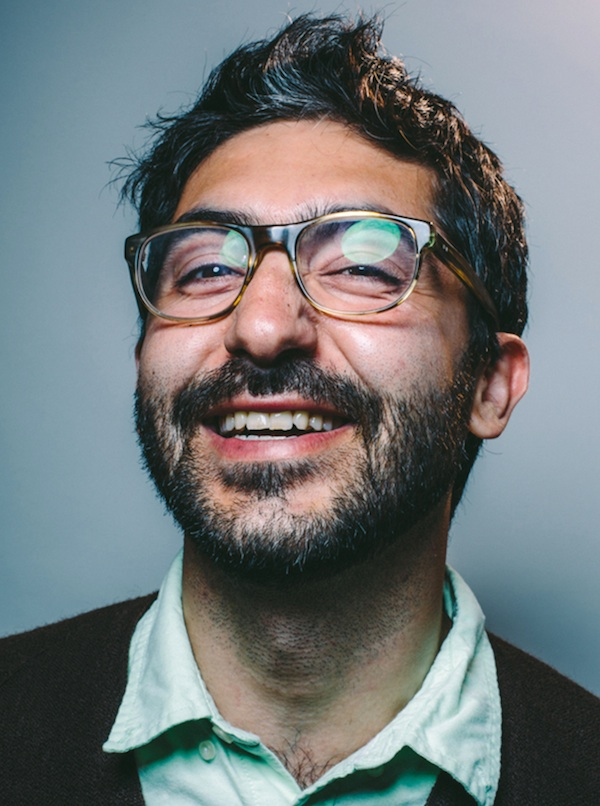
\includegraphics[width=3cm]{momeni-800.jpg}
  \caption{\textbf{Ali Momeni} is a builder, composer and performer interested in using technology to bring people together. His work makes use of all manners of technology to explore the social lives of objects and their embeded performative qualities, and how computation can give us a more intimate understanding of the world around us. His creative output ranges from kinetic sculptures and sound installations, to urban interventions, music theater performance, and large scale projection performances and writing. He especially likes working with plants and animals, and his favorite projects are collaborative, transnational, and transgenerational.}
\end{figure}

\begin{figure}[H]
  \sidecaption[t]
  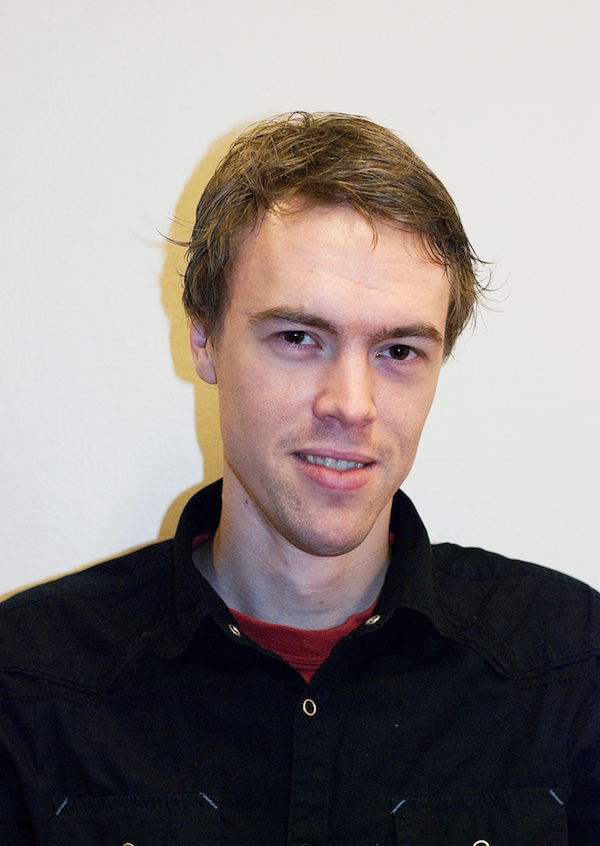
\includegraphics[width=3cm]{nymoen-800.jpg}
  \caption{\textbf{Kristian Nymoen} is Associate Professor in music technology at the University of Oslo. His research interests covers a range of different areas including development of new musical instruments, motion capture technologies, analysis of music-related body motion, machine learning and music cognition.}
\end{figure}

\begin{figure}[H]
  \sidecaption[t]
  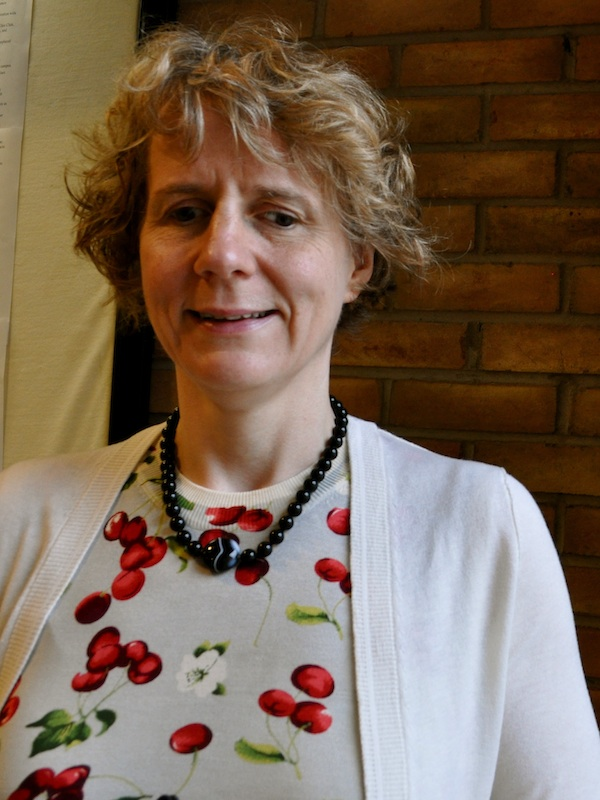
\includegraphics[width=3cm]{omodhrain-800.jpg}
  \caption{\textbf{Sile O'Modhrain} holds a joint appointment in the School of Information and in the School of Music, Theatre and Dance at the University of Michigan. She received her Ph. from Stanford's Center for Computer Research in Music and Acoustics (CCRMA). Her research focuses on human-computer interaction, especially interfaces incorporating haptic and auditory feedback.}
\end{figure}

\begin{figure}[H]
  \sidecaption[t]
  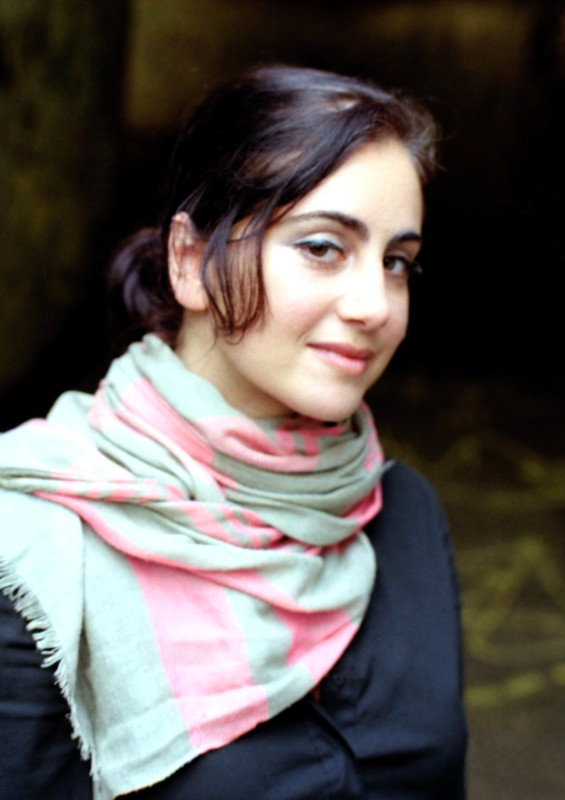
\includegraphics[width=3cm]{ouzounian-800.jpg}
  \caption{\textbf{Gascia Ouzounian} is Senior Lecturer in Music at Queen's University Belfast. As a musicologist and violinist her work is situated in relation to experimental music traditions of the last century. Her research examines topics including the history of spatial audio, site-specific sound art, multichannel electroacoustic composition, and the intersection of experimental music and visual arts traditions. Ouzounian's articles appear in many of the leading journals of contemporary music, including Computer Music Journal, Contemporary Music Review, Organised Sound, and Leonardo Music Journal. With the architect Sarah Lappin she co-directs the interdisciplinary research group Recomposing the City: Sound Art \& Urban Architecture.}
\end{figure}

\begin{figure}[H]
 \sidecaption[t]
 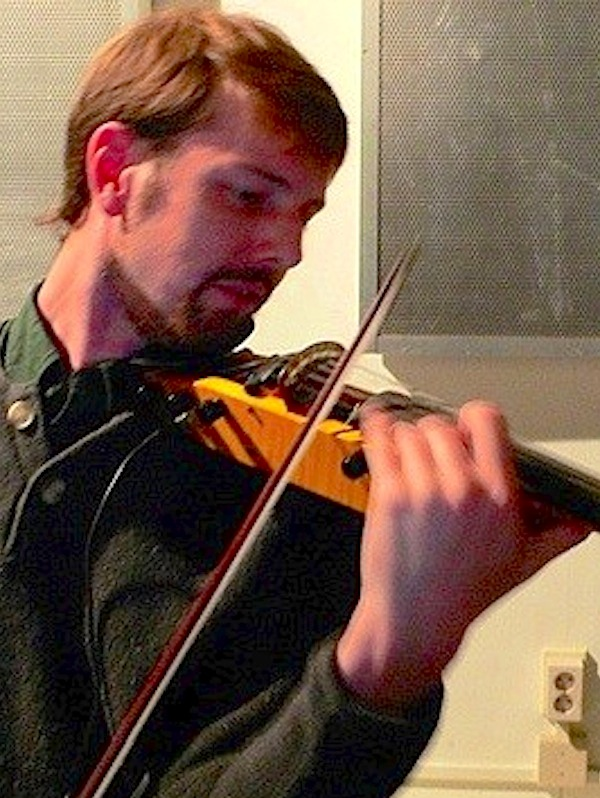
\includegraphics[width=3cm]{overholt-800.jpg}
 \caption{\textbf{Dan Overholt} is Associate Professor at Aalborg University Copenhagen, Department of Architecture, Design and Media Technology. His research and teaching are centered within the Medialogy, and Sound \& Music Computing programs there. Prior, he was a postdoctoral fellow in the Media Arts and Technology (MAT) program and Lecturer / Researcher at the Center for Research in Electronic Art Technology (CREATE) at UC Santa Barbara. His dissertation, entitled \lq Musical Interface Technology: Multimodal Control of Multidimensional Parameter Spaces for Electroacoustic Music Performance,\rq is the result of a long-term focus on the development of advanced technologies for interactive interfaces, and novel audio signal processing algorithms.}
\end{figure}

\begin{figure}[H]
  \sidecaption[t]
  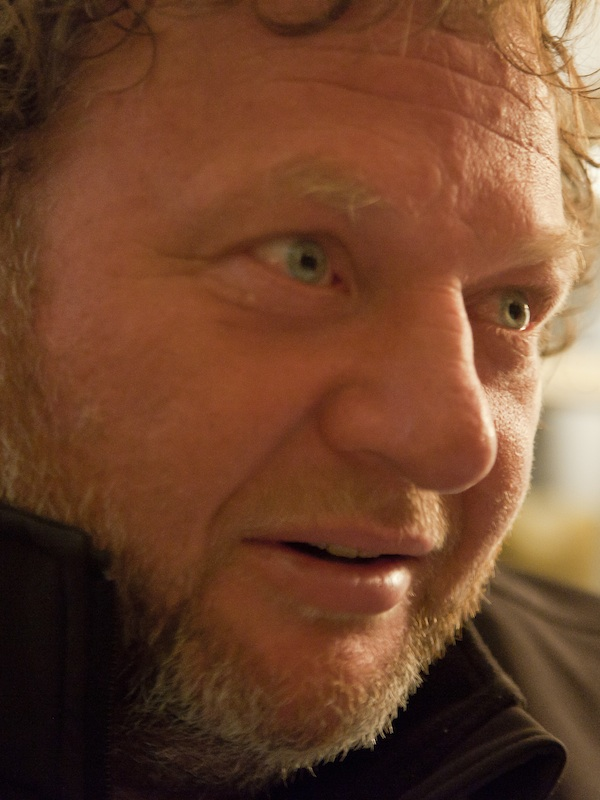
\includegraphics[width=3cm]{paine-800.jpg}
  \caption{\textbf{Garth Paine} is fascinated with sound as an exhibitable object, enquiries into the materiality of sound and interaction inspired several interactive responsive environments in the 1990's where the inhabitant generated the sonic landscape through presence and behavior. More recent fixed media compositions and interactive music scores for dance, generated through video tracking and or bio-sensing of the dancers have been presented throughout Australia, Europe, Japan, USA, Asia and Australia. His work on a NIME taxonomy %\footnote{\url{http://vipre.uws.edu.au/dmi/}} 
  was one of the initial efforts in the field.}
\end{figure}

\begin{figure}[H]
  \sidecaption[t]
  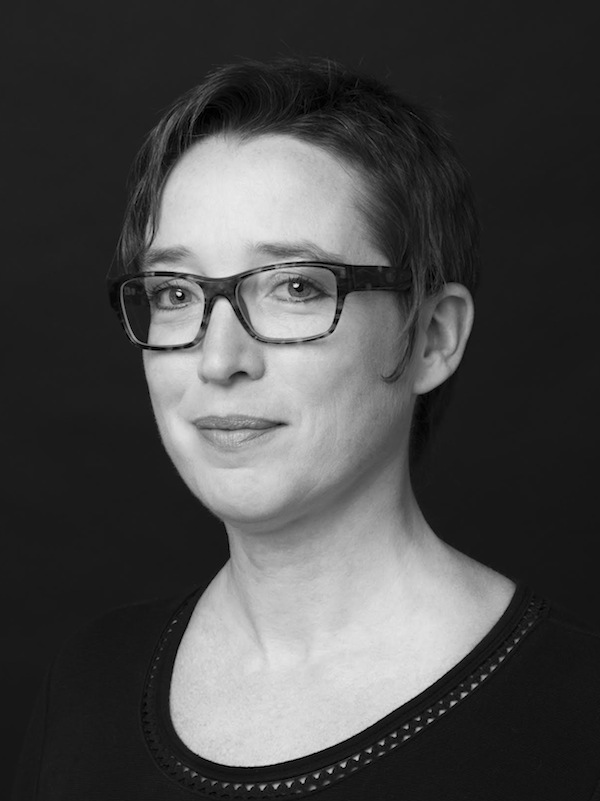
\includegraphics[width=3cm]{palacio-quintin-800.jpg}
  \caption{\textbf{Cl\'eo Palacio-Quintin} is a flutist-improviser-composer. Constantly seeking new means of expression and eager to create, she takes part in many premieres as well as improvisational multidisciplinary performances, and composes instrumental and electro-acoustic music for various ensembles and media works. Since 1999, she has been developing the hyper-flutes. Interfaced to a computer by means of electronic sensors, these enhanced flutes enable her to compose novel interactive music and control live video processing. She is the first woman to earn a Doctorate in Electro-Acoustic Composition from the Universit\'e de Montr\'eal (2012) and collaborates with the Centre for Interdisciplinary Research in Music Media and Technology (CIRMMT).}
\end{figure}

\begin{figure}[H]
  \sidecaption[t]
  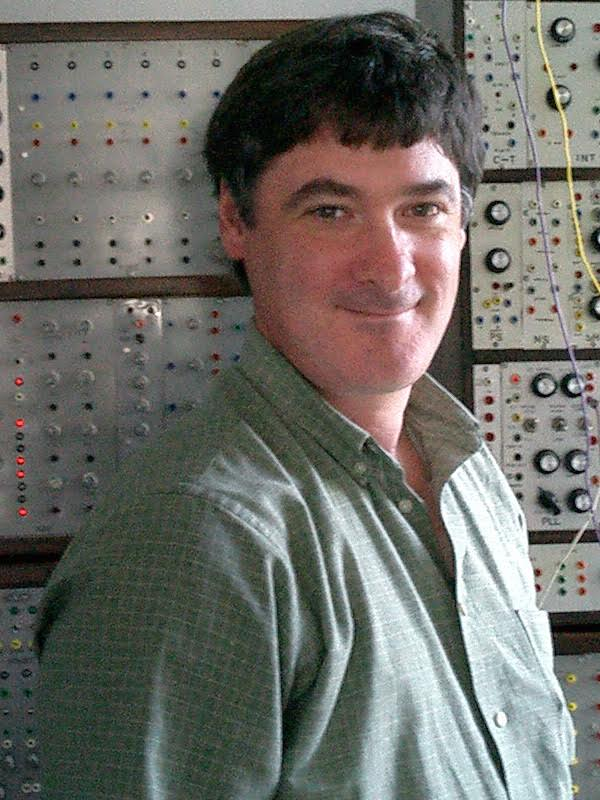
\includegraphics[width=3cm]{paradiso-800.jpg}
  \caption{\textbf{Joe Paradiso} is the Alexander W. Dreyfoos (1954) Professor in Media Arts and Sciences at the MIT Media Lab, where he directs the Responsive Environments group. He received his PhD in Physics from MIT in 1981 and a BSEE from Tufts University in 1977, and joined the Media Lab in 1994. He has been designing and building electronic music systems since 1974. His current research explores how sensor networks augment and mediate human experience, interaction and perception---encompassing wireless sensing systems, wearable and body sensor networks, energy harvesting and power management for embedded sensors, ubiquitous and pervasive computing, human-computer interfaces, and interactive media.}
\end{figure}

\begin{figure}[H]
  \sidecaption[t]
  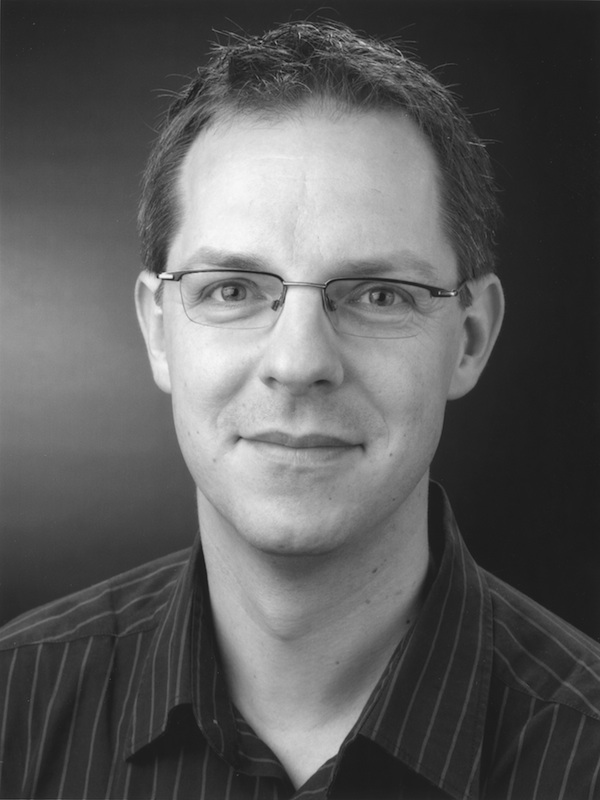
\includegraphics[width=3cm]{poepel-800.jpg}
  \caption{\textbf{Cornelius Poepel} is a violist, audio designer, and sound artist. Since 2008, he is Professor of Audio Producing at Ansbach University of Applied Sciences. He received his PhD from the University of Birmingham, UK working on audio signal-driven sound synthesis. After working at ZKM Karlsruhe he joined the faculty of the Academy for Media Arts Cologne. He has performed world wide as orchestra-violist and in experimental performances using the laptop, synthesizer, and acoustic instruments.}
\end{figure}

\begin{figure}[H]
  \sidecaption[t]
  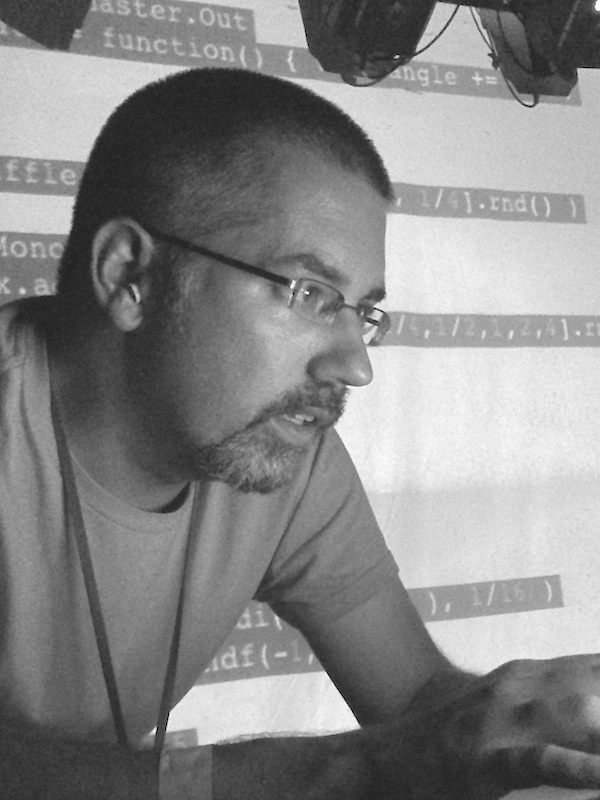
\includegraphics[width=3cm]{roberts-800.jpg}
  \caption{\textbf{Charlie Roberts} is an Assistant Professor in the School of Interactive Games and Media at the Rochester Institute of Technology, where he researches human-centered computing in digital arts practice. He is the lead designer and developer of \textit{Gibber}, a creative coding environment for the browser, and has performed with it throughout the US, UK and Asia in the experimental performance genre known as live coding.}
\end{figure}

\begin{figure}[H]
  \sidecaption[t]
  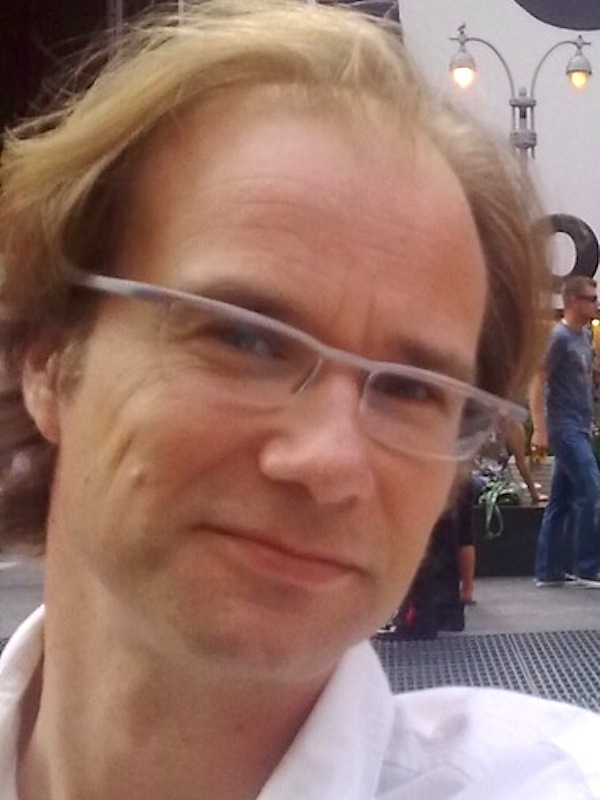
\includegraphics[width=3cm]{schnell-800.jpg}
  \caption{\textbf{Norbert Schnell} is a researcher and developer focussing on real-time interactive digital audio processing and interaction design. Together with his colleagues of the Sound Music Movement Interaction team at IRCAM in Paris he develops technologies and interaction scenarios on the frontiers between music listening and music performance. In 2006 he chaired the 6\textsuperscript{th} International Conference on New Interfaces for Musical Expression (NIME). He currently coordinates the CoSiMa research project that investigates collaborative musical interaction scenarios using web and mobile technologies.}
\end{figure}


\begin{figure}[H]
  \sidecaption[t]
  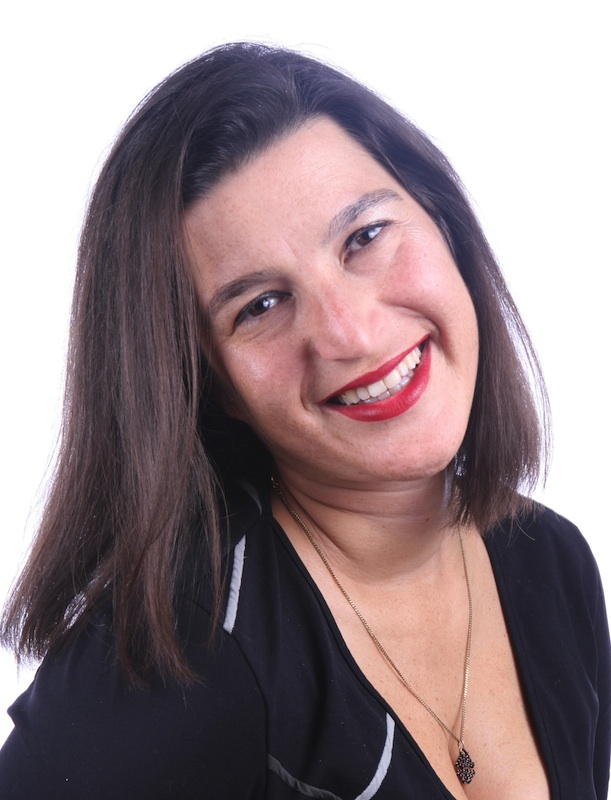
\includegraphics[width=3cm]{serafin-800.jpg}
  \caption{\textbf{Stefania Serafin} is Professor with special responsibilities in sound for multimodal environments at Aalborg University Copenhagen. She received a PhD degree in computer-based music theory and acoustics from Stanford University, in 2004, and a Master in Acoustics, computer science and signal processing applied to music from IRCAM, in 1997. She is the president of the Sound and Music Computing Association, and the Vice-President for the International Computer Music Association. She has extensively published in numerous international journals and conferences.}
\end{figure}

\begin{figure}[H]
  \sidecaption[t]
  \includegraphics[width=3cm]{smallwood-800.jpg}
  \caption{\textbf{Scott Smallwood} is a sound artist, composer, and musician who creates works inspired by discovered textures and forms, through a practice of listening, field recording, and sonic improvisation. He designs experimental electronic instruments and software, as well as sound installations and site-specific performance scenarios. He performs as one-half of the laptop/electronic duo Evidence (with Stephan Moore), and currently lives in Edmonton, Alberta, where he teaches composition, improvisation, and electroacoustic music at the University of Alberta.}
\end{figure}

\begin{figure}[H]
  \sidecaption[t]
  \includegraphics[width=3cm]{stapleton-800.jpg}
  \caption{\textbf{Paul Stapleton} is an improviser, sound artist, instrument designer and critical theorist originally from Southern California. He is currently a Senior Lecturer at the Sonic Arts Research Centre, Queen's University Belfast, where he teaches and supervises research in performance technologies, improvisation and site-specific sound art. His album FAUNA with saxophonist Simon Rose has received acclaim from critics such as Ken Waxman (Jazzword), Jean-Michel Van Schouwburg (Orynx), Mark Corroto (All About Jazz), and Marc Medwin (New York City Jazz Record). Paul also co-directs the Translating Improvisation research group with Sara Ramshaw and the QUBe music collective with Steve Davis.}
\end{figure}

\begin{figure}[H]
  \sidecaption[t]
  \includegraphics[width=3cm]{tahiroglu-800.jpg}
  \caption{\textbf{Koray Tahiro\u{g}lu} is a research fellow, musician and lecturer in the Department of Media at the Aalto University School of Arts, Design and Architecture, Finland. He is the founder and head of the SOPI (Sound and Physical Interaction) research group. He practices art as a researcher focusing on embodied approaches to sound and music interaction, as well as a performer of live electronic music. Since 2004 he has also been teaching workshops and courses introducing artistic strategies and methodologies for creating interactive music. Tahiro\u{g}lu has performed experimental music in collaboration as well as in solo performances in Europe and North America.}
\end{figure}

\begin{figure}[H]
  \sidecaption[t]
  \includegraphics[width=3cm]{tanaka-800.jpg}
  \caption{\textbf{Atau Tanaka} is Professor of Media Computing at Goldsmiths. He has previously been Chair of Digital Media at Newcastle University (UK), and researcher at Sony Computer Science Laboratory (CSL) Paris. During his doctorate at Stanford University's CCRMA, he was awarded the Prix de Paris to conduct research at IRCAM. He has been artistic ambassador for Apple Computer, mentor at NESTA, and Artistic Co-Director of STEIM in Amsterdam. He has performed his work using physiological musical interfaces across Europe, in Japan, and the US. His research has been funded by the RCUK, ANR (France), and the European Research Council.}
\end{figure}

\begin{figure}[H]
  \sidecaption[t]
  \includegraphics[width=3cm]{trevino-800.jpg}
  \caption{\textbf{Jeffrey Trevi\~no} is Assistant Professor of Music and Technology at Colorado College. His research and creative practice focus on feedback between symbolic representation, human-computer interaction, and sonic creativity, with an emphasis on the way novel technologies and representations impact established conventions of theory and practice. As a composer, his orchestral, chamber, and solo acoustic and electroacoustic works have been premiered internationally by acclaimed soloists and ensembles. As a music technology researcher and software developer, Trevi\~no contributes code to the nCoda and Abjad Python music notation projects and is a member of the W3C Music Notation Community group.}
\end{figure}

\begin{figure}[H]
  \sidecaption[t]
  \includegraphics[width=3cm]{trueman-800.jpg}
  \caption{\textbf{Dan Trueman} is a composer, fiddler, and electronic musician. His work has been recognized by the Guggenheim and MacArthur Foundations, the Barlow Endowment, the Fulbright Commission, the American Composers Forum, the American Council of Learned Societies, Meet the Composer, among others. He is Professor of Music and Director of the Princeton Sound Kitchen at Princeton University, where he teaches counterpoint, electronic music, and composition.}
\end{figure}

\begin{figure}[H]
  \sidecaption[t]
  \includegraphics[width=3cm]{van-nort-800.jpg}
  \caption{\textbf{Doug Van Nort} is an artist, researcher, composer and performer. His work is concerned with questions surrounding distributed agency and sensorial immersion in technologically-mediated performance. He creates works that integrate improvisation and collective performance with machine agents, interactive systems and experiences of telepresence. He often performs solo as well as with a wide array of artists across musical styles and artistic media. Van Nort is Canada Research Chair in Digital Performance in the School of Arts, Media, Performance and Design (AMPD) at York University, where he is founding director of the DisPerSion Lab.}
\end{figure}

\begin{figure}[H]
  \sidecaption[t]
  \includegraphics[width=3cm]{visi-800.jpg}
  \caption{\textbf{Federico Visi} is a researcher, composer and performer. He is currently based in Plymouth (UK) where he is conducting his doctoral research at the Interdisciplinary Centre for Computer Music Research (ICCMR) focusing on body movement in performances with traditional musical instruments. He has composed music for films and installations, performed live in solo sets, with bands and in contemporary theatre and dance performances and presented his research at several international conferences. He is working on collaborative, interdisciplinary projects with researchers in Europe (Ghent University, University of Bologna), North America (NYU, UCLA) and South America (Universidade Federal do Rio Grande do Sul).}
\end{figure}


\begin{figure}[H]
  \sidecaption[t]
  \includegraphics[width=3cm]{verplank-800.jpg}
  \caption{\textbf{Bill Verplank} is Lecturer at Stanford University (CCRMA, CS, ME) where he has taught and done research since retiring from Interval Research ('92--'00), IDTwo ('86--'92) and Xerox ('78--'86). He teaches one or two weeks a year at Copenhagen Institute of Interaction Design, and before that was on the Steering Committee of Interaction Design Institute Ivrea. His education is in man-machine systems (MIT PhD '71) and mechanical engineering (Stanford BS '65). With Sheridan he pioneered ``man-machine systems,'' Xerox ``user-interface design'' with Bill Moggridge ``interaction design,'' and with Max Mathews ``new interfaces for musical expression.''}
\end{figure}

\begin{figure}[H]
  \sidecaption[t]
  \includegraphics[width=3cm]{wakefield-800.jpg}
  \caption{\textbf{Graham Wakefield's} research-creation is founded upon a trans-disciplinary academic training in interactive art, music, mathematics and philosophy, partnered with an international exhibition record and extensive professional software engineering for creative coding in audio-visual, interactive and immersive virtual and augmented-reality media. Currently Assistant Professor in Digital Media, Visual Art \& Art History and Canada Research Chair in Interactive Information Visualization at York University, Canada, he previously held research appointments at KAIST, Korea, and in the AlloSphere Research Group at the University of California, Santa Barbara. He is also co-author of the widely-used Gen extension for Max/MSP/Jitter.}
\end{figure}

\begin{figure}[H]
  \sidecaption[t]
  \includegraphics[width=3cm]{wanderley-800.jpg}
  \caption{\textbf{Marcelo Mortensen Wanderley} holds a PhD degree from Universit\'e Pierre et Marie Curie (Paris VI), France, on acoustics, signal processing, and computer science applied to music. Prof. Wanderley chaired the 2003 International Conference on New Interfaces for Musical Expression, co-edited the electronic book ``Trends in Gestural Control of Music,'' IRCAM, 2000, and co-authored the textbook, ``New Digital Musical Instruments: Control and Interaction Beyond the Keyboard'', A-R Editions, 2006. He is William Dawson Scholar and Professor of Music Technology at the Schulich School of Music, McGill University, Montreal, Quebec, Canada.}
\end{figure}

\begin{figure}[H]
  \sidecaption[t]
  \includegraphics[width=3cm]{wang-800.jpg}
  \caption{\textbf{Ge Wang} investigates artful design of interactive music software, programming languages, new computer-mediated instruments, expressive mobile and social music apps, as well as the evolution of laptop orchestras and education at the intersection of computer science and music. He is Assistant Professor at Stanford University's Center for Computer Research in Music and Acoustics (CCRMA), and the co-founder of Smule (reaching over 125 million users). Ge is the author of the ChucK audio programming language (with Perry Cook), the founding director of the Stanford Laptop Orchestra (SLOrk), and the designer of the iPhone's Ocarina and Magic Piano.}
\end{figure}

\begin{figure}[H]
  \sidecaption[t]
  \includegraphics[width=3cm]{wessel-800.jpg}
  \caption{\textbf{David Wessel} (1942--2014) was the founding Director of UC Berkeley's Center for New Music and Audio Technologies (CNMAT) from its 1988 founding until his untimely passing. He performed as a professional jazz drummer in high school, earned a BS in mathematical statistics from the University of Illinois in 1964 and a PhD in mathematical psychology at Stanford University in 1972, and conducted research and taught at SF State University and Michigan State University before working at IRCAM and founding CNMAT.}
\end{figure}

\begin{figure}[H]
  \sidecaption[t]
  \includegraphics[width=3cm]{wright-800.jpg}
  \caption{\textbf{Matthew Wright} is a computer music researcher, improvising composer/performer, musical ensemble leader, and media systems designer. He is currently Technical Director of Stanford's Center for Computer Research in Music and Acoustics (CCRMA), and was previously Research Director of UC Santa Barbara's Center for Research in Electronic Arts and Technology (CREATE) where his CREATE Ensemble provided a venue, users, and performance opportunities for early versions of Gibber. His research interests include interactive systems, musical rhythm, new interfaces for musical expression, sound synthesis, sonification and visualization, interactive audiovisual system design, musical networking, sound in space, and computational ethnomusicology.}
\end{figure}

\begin{figure}[H]
  \sidecaption[t]
  \includegraphics[width=3cm]{young-800.jpg}
  \caption{\textbf{Diana Young} received her BS in Electrical Engineering and B.A. in Music from Johns Hopkins University, and her Performer's Certificate in Violin from the Peabody Conservatory of Music. She earned her M.S. and PhD from the MIT Media Laboratory for her research on measurement of bowed string performance parameters. In her postdoctoral work at MIT she contributed to the development of measurement systems for active lower limb prostheses. Most recently, her interests in human motion and the development of HCI for skill acquisition lead her to the Wyss Institute at Harvard as a Technology Development Fellow.}
  \end{figure}

%
% N.B. What do we do about the 'Biomuse Trio' Bio?
%
%%\begin{figure}[H]
%. \sidecaption[t]
% % \includegraphics[width=3cm]{Marcelo_NIME_800.jpg}
%. \caption{\textbf{The Biomuse Trio] (R.~Benjamin Knapp, Eric Lyon, Gascia Ouzounian) was formed in 2008 to perform computer chamber music integrating performance, laptop processing of sound and the transduction of bio-signals for the control of musical gesture. The work of the ensemble encompasses hardware design, audio signal processing, bio-signal processing, composition, improvisation and gesture choreography. The Biomuse Trio has performed and lectured across North America and Europe, including at BEAM Festival, CHI, Diapason Gallery, Green Man Festival, Issue Project Room, NIME, Science Gallery Dublin, STEIM and TheatreLab NYC.}
%%\end{figure}

\end{authbio}
